\documentclass[12pt]{article}

\usepackage{sbc-template}
\usepackage{graphicx,url}
\usepackage[utf8]{inputenc}
\usepackage[brazil]{babel}
%\usepackage[latin1]{inputenc}  
\usepackage{graphicx}
\usepackage{caption}
\usepackage{subcaption}
\usepackage{tabularx}
\usepackage{float}
\usepackage{array}
     
\sloppy

\title{Usabilidade e Acessibilidade Digital para Idosos: Uma Avaliação do Aplicativo ``Meu SUS Digital''}

\author{Samantha Vitória Moura da Silva\inst{1}, João Victor R. Lisboa\inst{1}, \\ João Pedro Vasconcelos de Lima\inst{1}, João Batista B. e Silva \inst{1}, Arthur Negrão Smith\inst{1}}


\address{Universidade Federal do Pará (UFPA) \\ 
Caixa Postal 479 – 66.075-110 – Belém – PA – Brasil
\
  \email{\{samantha.silva, joao.lisboa, joao.vasconcelos,}
    \vspace{-0.4cm}
    \email{joao.barbosa.silva, arthur.smith\}@icen.ufpa.br}
}

\begin{document} 

\maketitle

9pp
\begin{abstractp}
This paper presents a usability and accessibility evaluation of the Meu SUS Digital application focused on the aging population, combining three complementary methods: Heuristic Evaluation, Usability Testing with real users, and the Semiotic Inspection Method (SIM). The Heuristic Evaluation identified 11 usability problems, six of which were classified as catastrophic, many of which were later confirmed during empirical testing with five participants aged between 52 and 70 years. Based on these findings, an interface redesign process was conducted, followed by a new usability test with a revised prototype, whose results indicated a partial resolution of the identified problems. The results reinforce the importance of multi-method evaluations in the development of inclusive government systems, particularly to ensure the autonomy of older users in accessing digital public services.
\end{abstract}
     
\begin{resumo} 
  Este artigo apresenta uma avaliação de usabilidade e acessibilidade do aplicativo Meu SUS Digital voltada ao público em processo de envelhecimento, combinando três métodos complementares: Avaliação Heurística, Teste de Usabilidade com usuários reais e Método de Inspeção Semiótica (MIS). A Avaliação Heurística identificou 11 problemas de usabilidade, sendo seis classificados como catastróficos, muitos dos quais foram posteriormente confirmados durante os testes empíricos com cinco participantes com idade entre 52 e 70 anos. A partir desses achados, foi conduzido um processo de redesign da interface, seguido de um novo teste de usabilidade com um protótipo revisado, cujos resultados indicaram uma resolução parcial dos problemas identificados. Os resultados reforçam a importância de avaliações multimétodo no desenvolvimento de sistemas governamentais inclusivos, especialmente para garantir a autonomia de usuários idosos no acesso a serviços públicos digitais.
\end{resumo}


\section{Introdução}

 O envelhecimento populacional é um fenômeno global que reformula as estruturas sociais, essa mudança também se reflete no cenário brasileiro, dados do \cite{ibge2022} demonstram esse avanço ao registrarem um aumento de quase 50\% no contingente de pessoas idosas em 2022, quando comparado ao censo de 2010. Diante do amadurecimento da população brasileira, torna-se cada vez mais perceptível a discussão sobre a necessidade de adaptação das esferas públicas e privadas para garantir a qualidade de vida, o bem-estar dessa parcela social, além buscar entender a inserção desse perfil etário nos escopos que formam a sociedade atual.

 Essa inserção torna-se ainda mais complexa  ao observar que a popularização da internet residencial marcou uma revolução global, transformando profundamente as relações econômicas, políticas e sociais. Diante desse cenário, a capacidade de adaptabilidade individual tornou-se um requisito indispensável para acompanhar as rápidas transformações impostas por essa tecnologia e a não adaptabilidade resulta na exclusão do indivíduo \cite{wiei}. Torna-se necessário, portanto, discutir de que maneira a população idosa vivencia essa realidade e enfrentando os desafios impostos por interfaces que frequentemente ignoram suas necessidades particulares \cite{alves2016tecnologias}.

 Para realizar o mapeamento das dificuldades encontradas por idosos, o seguinte trabalho utilizou de diversas ferramentas e conceitos próprios da área da Interação Humano Computador (IHC) para identificar possíveis problemas de interface, o objeto de estudo definido foi a aplicação governamental Meu SUS Digital \cite{meususdigital}, utilizada para acessar informações informações médicas, históricos de vacinação e agendamentos de serviços públicos de saúde. Sendo assim, a metodologia aplicada no trabalho consistiu, primeiramente, na realização de uma avaliação heurística desenvolvida a partir de um cenário definido anteriormente, em seguida, conduziu-se um teste de usabilidade prático com usuários reais na faixa etária de 52 a 70 anos e, por fim,  aplicou-se o Método de Inspeção Semiótica (MIS), com a finalidade de avaliar a qualidade da metacomunicação e compreender como o aplicativo se comunica com seus usuários.

Os resultados evidenciaram a existência de diversos problemas de usabilidade, muitos dos quais confirmados empiricamente durante os testes com usuários reais, tais achados nortearam o processo de \textit{redesign} da interface, seguido de uma nova validação junto a usuários, cujos resultados indicaram uma mitigação parcial das barreiras identificadas.

 Este artigo está organizado da seguinte forma: a Seção 2 apresenta a fundamentação teórica que embasa os métodos utilizados; a Seção 3 descreve a metodologia aplicada em cada etapa da pesquisa; a Seção 4 discute os resultados obtidos; e a Seção 5 apresenta as considerações finais do trabalho.
 
\section{Fundamentação Teórica} \label{sec:fundamentacao}

Esta seção apresenta conceitos relevantes para o desenvolvimento desse trabalho, elucidando conceitos introdutórios da Interação Humano-Computador, além dos métodos de inspeção e de observação utilizados na avaliação do sistema. 


\subsection{Interação Humano-Computador}
\label{sec:ihc}

A área de Interação Humano-Computador (IHC) dedica-se a estudar e compreender a interação das pessoas com a tecnologia, envolvendo a influência de aspectos culturais, sociais e organizacionais no desenvolvimento e no uso de sistemas computacionais. Além disso, essa área de estudo se beneficia de métodos e conhecimentos que transcendem a computação, incorporando contribuições de disciplinas como a psicologia, a sociologia e a antropologia \cite{barbosa2010ihc}.

%O objeto de estudo de IHC ampara-se em princípios focados na usabilidade e na experiência do usuário, denominados qualidades de IHC , a implementação de tais princípios visa estabelecer sistemas com melhor facilidade de uso e de aprendizado, os principais critérios observados são \cite{barbosa2010ihc}: 

%\begin{itemize}
   % \item \textbf{Usabilidade:} trata-se do uso de um produto para o usuário atingir um objetivo específico com eficiência, eficácia e satisfação do uso \cite{iso9241}. 
    %\item \textbf{Experiência do Usuário}: destaca que o contato do consumidor com a interface possui questões emocionais e subjetivas que devem ser levadas em consideração durante o projeto \cite{barbosa2010ihc}.
    %\item \textbf{Acessibilidade:} Garante que o usuário possua plena independência durante o uso da ferramenta, removendo barreiras para que diferentes perfis de pessoas consigam interagir com o sistema com autonomia \cite{barbosa2010ihc}.
     %\item \textbf{Comunicabilidade:} Ressalta a capacidade do designer de possuir uma interpretação sobre o usuário e estabelecer uma comunicação por meio da interface, a qual deve ser utilizada para auxiliar o receptor na manipulação e no entendimento da ferramenta \cite{barbosa2010ihc}.

    
%\end{itemize}

\subsection{Acessibilidade Digital e os Desafios da População Idosa} \label{acessibilidade_idoso}

A acessibilidade digital é o termo que designa a implementação de um conjunto de soluções que visa ampliar o acesso a tecnologias interativas, permitindo que estas se adaptem às necessidades, capacidades e preferências de qualquer indivíduo, independentemente de suas condições físicas, motoras, visuais, auditivas ou cognitivas. Isto é, o objetivo principal da aplicação da acessibilidade é garantir que qualquer indivíduo utilize as tecnologias com autonomia e independência \cite{brasil_acessibilidade_digital}. 

Ao ampliar a discussão da acessibilidade para a população idosa, identifica-se a diversidade de disfunções que devem ser levadas em consideração na criação de sistemas interativos, visto que esse público possui especificidades altamente diversas. Dito isso, destaca-se que o envelhecimento impacta, principalmente, os aspectos visuais, cognitivos e motores dos sujeitos, evidenciando que a construção da acessibilidade digital aplica repertório não só tecnológico, mas também social e biológico \cite{barbosa2010ihc}.

\subsection{Avaliação Heurística e as Diretrizes de Nielsen} \label{subsec:heuristica}

A avaliação heurística consiste em um método de inspeção de usabilidade realizado por especialistas, com o intuito de identificar problemas de interface. A inspeção é feita utilizando as heurísticas de usabilidade propostas por Jakob Nielsen, as quais funcionam como guias na promoção da qualidade do produto e da facilidade de uso do sistema para os usuários.

As heurísticas de Nielsen se baseiam em 10 princípios gerais para a interface do usuário, sendo amplamente utilizadas como diretrizes para aperfeiçoar a experiência do usuário, as quais são sintetizadas a seguir \cite{nielsen1994heuristic}:

\begin{enumerate}
    \item \textbf{Visibilidade do status do sistema;} %O usuário deve ser informado sobre o status do sistema de forma contínua e em tempo útil;
    \item \textbf{Correspondência entre o sistema e o mundo real;} %A interface deve adotar termos, frases e conceitos familiares, alinhados ao dia a dia do usuário;
    \item \textbf{Controle e liberdade do usuário;} %Na ocorrência de um erro ou arrependimento, o sistema deve oferecer uma "saída de emergência" clara, permitindo desfazer ou refazer a ação de forma simples;
    \item \textbf{Consistência e padrões;} %O sistema deve seguir convenções e padrões já estabelecidos, evitando que o usuário precise adivinhar se palavras ou ações diferentes significam a mesma coisa;
    \item \textbf{Prevenção de erros;}% Mais importante do que emitir boas mensagens de erro é projetar a interface para eliminar condições propensas a falhas ou solicitar confirmações antes que ações críticas sejam executadas;
    \item \textbf{Reconhecimento em vez de memorização;} %A interface deve tornar objetos, ações e opções visíveis, reduzindo a carga de memória do usuário ao dispensar a necessidade de lembrar informações de uma tela para outra;
    \item \textbf{Flexibilidade e eficiência de uso;} %O sistema deve ser intuitivo para usuários iniciantes e, simultaneamente, oferecer aceleradores e atalhos ocultos que otimizem a navegação de usuários experientes;
    \item \textbf{Estética e design minimalista;} %Os diálogos não devem conter informações irrelevantes ou raramente necessárias, visto que cada unidade extra de informação compete com as dados essenciais e diminui sua visibilidade;
    \item \textbf{Ajuda aos usuários para reconhecer, diagnosticar e recuperar-se de erros;} %As mensagens de erro devem ser expressas em linguagem clara (sem códigos), indicar precisamente o problema e sugerir uma solução construtiva;
    \item \textbf{Ajuda e documentação.} %Embora seja preferível que o sistema possa ser usado sem documentação, pode ser necessário fornecer informações de suporte que sejam fáceis de pesquisar, focadas nas tarefas do usuário e concisas.
\end{enumerate}
\subsection{Teste de usabilidade} \label{subsec:teste_usab}

O teste de usabilidade é um método de avaliação por observação, no qual, diferentemente da avaliação heurística que envolve apenas especialistas, a análise é realizada a partir da observação direta de como o usuário manipula a aplicação. Diante disso, a execução dessa avaliação é de suma importância para identificar falhas reais no produto e compreender o comportamento dos usuários, fornecendo subsídios concretos para o aprimoramento contínuo da interface. \cite{moran2019usability}


Segundo a norma ISO 9241-11 \cite{iso9241}, a usabilidade de uma aplicação está diretamente relacionada à capacidade do usuário de atingir seus objetivos com eficácia, eficiência e satisfação em um contexto de uso determinado. Diante disso, na realização de testes com o usuário, a observação e a mensuração dessas métricas tornam-se imprescindíveis para validar as experiências do usuário, além de identificar inconsistências no produto. Dito isso, a conceituação de tais medidas são descritas a seguir \cite{cybis2015ergonomia}: 
\begin{itemize}
    \item \textbf{Eficácia:} refere-se a capacidade do usuário atingir o objetivo pretendido com precisão e completude ao interagir com o sistema.No contexto do teste, ela é mensurada pela taxa de sucesso na conclusão das tarefas propostas, determinando se o participante conseguiu ou não finalizar o fluxo planejado de forma correta; 
    \item \textbf{Eficiência:} abrange a relação entre os resultados alcançados com os recursos utilizados (como tempo gasto, quantidade de cliques e esforço cognitivo) para a conclusão de uma determinada tarefa; 
   \item \textbf{Satisfação:} é a métrica que considera o nível de conforto, aceitação e confiança que o usuário possui ao interagir com o sistema, sendo amplamente mensurada a partir de capturas verbais do participante durante a interação com a ferramenta e da aplicação de questionários pós-teste;
\end{itemize}

\subsection{Engenharia Semiótica e Método de Inspeção Semiótica (MIS)} \label{subsec:eng_semiotica}

A Engenharia Semiótica é uma teoria de Interação Humano-Computador (IHC) proposta por Clarisse Sieckenius de Souza,  a sua fundamentação destaca que o contato do usuário com a interface não se limita ao mero manuseio de uma máquina, mas constitui, fundamentalmente, um processo de comunicação entre o projetista (\textit{designer}) e o usuário final, evidenciando  o sistema como um artefato de metacomunicação, por meio do qual o criador transmite ao usuário suas próprias percepções sobre o produto, tais como: quem é o público-alvo do sistema, quais necessidades daquele usuário a ferramenta visa suprir e de que maneira o sistema deve ser operado para alcançar tais objetivos \cite{desouza2005}. 

Vale destacar que essa comunicação é realizada por meio do uso de signos (palavras, ícones, menus, comportamentos) e da resposta desses elementos a cada interação do receptor. Diante da relevância dos signos na construção da interface, o Método de Inspeção Semiótica (MIS) surge como um método de inspeção conduzida por especialista, na qual possui como objetivo analisar os signos e suas respectivas respostas, dessa forma, avaliando a comunicabilidade do sistema \cite{desouza2005}.

 \section{Metodologia} \label{sec:metodologia}
 Esta seção detalha o percurso metodológico seguido durante o desenvolvimento do trabalho, destacando-se a aplicação de uma abordagem mista de avaliação (qualitativa e quantitativa).Dessa forma, para atender aos objetivos do estudo, o procedimento foi estruturado de forma sequencial em cinco etapas principais: três avaliações complementares da interface do aplicativo de bem-estar Meu SUS Digital,além do processo de redesign e da validação final por meio de prototipação. 
 
\subsection{Objeto de Estudo e Participantes} \label{sec:objeto_participantes}
O objeto de estudo selecionado foi o aplicativo governamental,o Meu SUS Digital, o qual consiste em uma plataforma desenvolvida para facilitar o acesso às informações voltadas à saúde, a partir da disponibilização de históricos de consultas e vacinas, por exemplo, para todos os cidadãos brasileiros \cite{meususdigital}. 

A partir disso, nota-se que a realização de avaliações nessa ferramenta torna-se indispensável, visto que, por se tratar de um sistema governamental, torna-se necessário garantir o acesso à diversidade de usuários, promovendo a inclusão digital de diferentes perfis \cite{barbosa2010ihc}.Por ser necessária essa diversificação, o estudo direcionado a idosos demonstra-se extremamente valioso, dado que esse grupo apresenta especificidades funcionais e cognitivas amplamente distintas entre si.


Para a realização dos testes empíricos de usabilidade, participaram da pesquisa cinco usuários voluntários que atendiam ao perfil de público-alvo delimitado, os participantes possuíam idade igual ou superior a 50 anos e experiência prévia no uso de dispositivos móveis. Inicialmente, pretendia-se realizar o estudo exclusivamente com indivíduos de 60 anos ou mais, entretanto, em razão das limitações de recrutamento dentro do período disponível para a pesquisa, optou-se por ampliar a faixa etária para incluir participantes a partir de 50 anos, preservando a proximidade com o público de interesse do estudo.

\subsection{Avaliação Heurística}
\label{sec:avaliacao_heuristica}

A avaliação heurística foi conduzida com o objetivo de identificar, de forma antecipada, possíveis problemas de usabilidade na interface do aplicativo Meu SUS Digital, a partir da análise de 3 avaliadores iniciantes, os quais utilizaram como guias as heurísticas de usabilidade propostas por Nielsen \cite{nielsen1994heuristic}.

Além disso, para  cada problema identificado, os avaliadores classificaram sua severidade de acordo com a escala proposta por Nielsen, que varia de 1 a 4, sendo:  1 (problema cosmético), 2 (problema de usabilidade menor), 3 (problema de usabilidade maior) e 4 (catástrofe de usabilidade) \cite{nielsen1994heuristic}. Essa classificação permitiu priorizar os problemas mais críticos identificados na interfaces, os quais foram priorizados no redesign. 

Vale ressaltar que, para auxiliar os avaliadores, houve a criação de uma persona e de um cenário de uso para orientar a realização da inspeção. A persona estabelecida consistiu em uma usuária do sexo feminino, com 70 anos de idade, professora da educação básica aposentada, que utiliza a internet predominantemente para interagir em redes sociais e necessita do auxílio de terceiros para lidar com novas tecnologias. A partir desse perfil, estipulou-se um cenário de uso com três metas principais de navegação no aplicativo:(i) realizar o login  (ii) exportar o comprovante de vacinação; (iii) verificar o histórico de consultas; e (iv) calcular o Índice de Massa Corporal (IMC) na funcionalidade ``Meu diário de saúde''. Assim, os avaliadores inspecionaram as telas simulando a jornada dessa persona, estimando a severidade dos problemas encontrados com base no impacto gerado para esse perfil de usuário.

\subsection{Teste de Usabilidade} \label{sub:test_usa}
O teste de usabilidade foi realizado com a finalidade de reafirmar os problemas achados durante a avaliação heurística. O teste foi aplicado em cinco usuários voluntários, com idade entre 52 e 70 anos que se encaixavam no perfil desejado ~\ref{sec:objeto_participantes}. Na aplicação do teste, os participantes foram instruídos a executar três tarefas principais no aplicativo móvel: (i) exportar o comprovante de vacinação; (ii) verificar o histórico de atendimentos; e (iii) calcular o Índice de Massa Corporal (IMC) na aba ``Meu Diário de Saúde''.

Vale ressaltar que, diferentemente do cenário projetado para a avaliação heurística, a etapa de autenticação foi removida do escopo de tarefas dos voluntários, essa modificação justificou-se por dois fatores principais: o aumento significativo do grau de dificuldade inicial da avaliação, caso o login fosse incluído, e a mitigação de riscos à segurança e à privacidade dos participantes, visto que o processo exigiria o fornecimento de credenciais reais (CPF e senha) da Conta gov.br. Dessa forma, os \textit{smartphones} utilizados nos testes foram disponibilizados e previamente preparados pela equipe de pesquisa, permitindo que os voluntários iniciassem a interação já devidamente autenticados na aplicação.

Ademais, antes da aplicação do teste, o moderador realizou a explicação a cerca das tarefas a serem realizadas, além de ressaltar que o foco da avaliação não seria o desempenho do indivíduo, mas sim a usabilidade da interface, destacando a inexistência de execução "correta ou "incorreta". A avaliação ocorreu da seguinte forma: para cada tarefa, foram registrados o grau de sucesso na execução, o total de erros cometidos, os tipos de erro e o tempo necessário para conclusão, a partir de observação direta durante a execução das tarefas.

\subsection{Método de Inspeção Semiótica (MIS)} \label{sub_MIS}

O Método de Inspeção Semiótica (MIS) foi aplicado com a finalidade de complementar os achados da avaliação heurística e do teste de usabilidade, investigando como a metacomunicação entre a equipe de design e o usuário final se manifesta por meio dos signos presentes na interface do aplicativo Meu SUS Digital, seguindo o percurso metodológico proposto por \cite{monsalve2011}. A aplicação do método foi estruturada em seis etapas: (i) preparação da inspeção, na qual foram definidas as fontes de informação e o escopo da jornada de navegação analisada; (ii) análise dos signos metalinguísticos; (iii) análise dos signos estáticos; (iv) análise dos signos dinâmicos; (v) comparação das metamensagens levantadas nas etapas anteriores; e (vi) avaliação da qualidade da comunicabilidade do sistema. O ponto de inspeção escolhido foi a funcionalidade ``Meu Diário de Saúde'', por concentrar os dois problemas classificados como catastróficos na avaliação heurística (Seção~\ref{sec:resultados_heuristica}).

\subsection{Processo de \textit{redesign}}\label{sub_redesign}
Para a criação das novas telas da interface, realizando as modificações necessárias nos problemas encontrados, utilizou-se a ferramenta Figma\footnote{https://www.figma.com/}, que permite o desenvolvimento de designs de forma colaborativa e facilita a criação de um protótipo clicável. Diante disso, buscou-se realizar capturas de tela do aplicativo "Meu SUS Digital" e utilizar trechos delas junto com novos elementos criados pela equipe para propor a nova interface.

Após isso, escolheu-se modificar três áreas do sistema, que se julgou serem as mais críticas, sendo elas: (I) exportar comprovante de vacinação, (II) pesquisar a função "IMC" na barra de pesquisa no menu e (III) registrar o IMC. Após feitas essas mudanças, definiu-se o fluxo dessas áreas e quais as funções desempenhadas pelos botões, para posteriormente testar com usuários.

\subsection{Teste de usabilidade com protótipo} \label{sub_usab_prototipo}
Após a implementação das modificações baseadas nos problemas identificados e elucidados nas etapas anteriores, aplicou-se um novo teste de usabilidade. Entretanto, o objetivo principal consistiu em avaliar se as alterações de fato proporcionaram uma melhoria significativa na experiência do usuário. Para isso, o teste foi conduzido com dois participantes acima de 60 anos, ambos alinhados ao perfil estabelecido para este trabalho.

Além disso, é importante frisar que, diferentemente da primeira rodada de testes de usabilidade, na qual havia um cenário muito mais extenso que possibilitava a livre navegação entre todas as telas, para a realização deste teste foram utilizados três fluxos de telas principais, não interligados, contemplando as três áreas do sistema anteriormente citadas. Assim, para a estruturação dos fluxos com base nos cenários estabelecidos, utilizou-se a ferramenta Figma para a construção de um protótipo clicável, como observado na Figura \ref{fig:fluxos-figma}.
\begin{figure}[h]
  \centering
  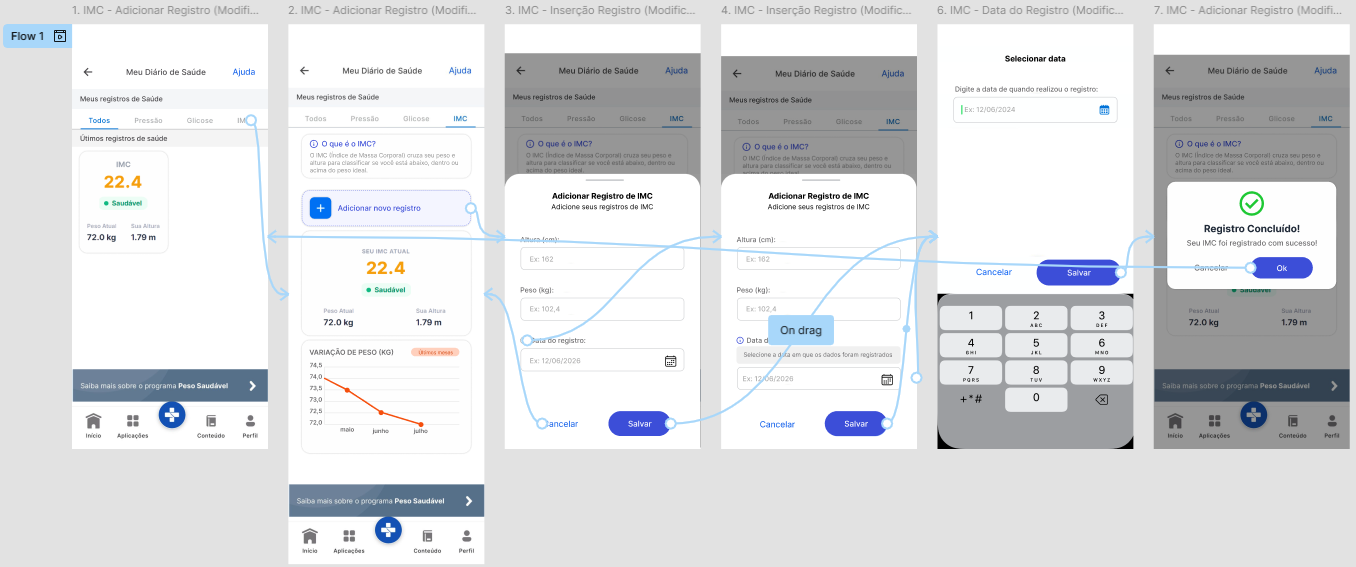
\includegraphics[width=\linewidth]{imagens/fluxos_figma.png}
  \caption{Criação do protótipo clicável}
  \label{fig:fluxos-figma}
\end{figure}

Para a execução dos testes baseados nos fluxos previamente determinados, escolheu-se um ambiente calmo e livre de interferências externas, minimizando possíveis distrações dos participantes. A interação com o protótipo ocorreu por meio da versão mobile do Figma em ambos os casos, que permitiu aproximar o protótipo de uma situação real. Por fim, utilizou-se um segundo dispositivo móvel para cronometrar o tempo de execução das tarefas, além de um caderno de notas para o registro das observações.

Outrossim, o entrevistador buscou evitar interferir durante a interação do usuário com a interface para não gerar resultados imprecisos ou errôneos, intervindo apenas quando necessário. Após a realização dos testes, realizou-se uma pequena entrevista não estruturada, utilizando técnicas como escuta ativa e \textit{Uh-uh prompt}, visando identificar se havia recomendações ou reclamações por parte do participante.

\section{Resultados} \label{resultados}
Nesta seção serão debatidos os resultados encontrados a partir das avaliações descritas na seção~\ref{sec:metodologia}. Inicialmente, serão apresentados os problemas de usabilidade encontrados por meio da avaliação heurística, seguidos dos resultados da aplicação dos testes de usabilidade realizados com os voluntários, a posteriori, são apresentados os resultados da aplicação do Método de Inspeção Semiótica (MIS). Diante da síntese desses achados, são descritos os problemas selecionados para o processo de redesign, bem como as alterações propostas na interface. Por fim, são apresentados os resultados do teste de usabilidade realizado com o protótipo redesenhado, com o objetivo de verificar se os problemas identificados anteriormente foram efetivamente solucionados.

 \subsection{Resultados da Avaliação Heurística} \label{sec:resultados_heuristica}

A avaliação foi realizada individualmente por cada avaliador, tanto pela versão mobile quanto pela versão web do aplicativo, sendo os resultados posteriormente discutidos e consolidados em conjunto. Ao todo, foram identificados 11 problemas de usabilidade, distribuídos nas quatro etapas avaliadas. Desses, 1 problema foi classificado como cosmético, 4 como grandes e 6 como catastróficos, segundo a escala de severidade de Nielsen. A Tabela~\ref{tab:heuristica} apresenta a relação completa dos problemas identificados, indicando a etapa em que ocorrem, a descrição do problema, as heurísticas violadas e a severidade atribuída a cada ocorrência.


\begin{table*}[htbp]
\centering
\footnotesize
\renewcommand{\arraystretch}{0.95}
\caption{Problemas identificados na Avaliação Heurística}
\label{tab:heuristica}
\begin{tabular}{|p{3.5cm}|p{7.5cm}|c|}
\hline
\textbf{Local/Etapa} & \textbf{Descrição do Problema} & \textbf{Heur.} / \textbf{Sev.} \\
\hline

Autenticação (login Gov.br) & 
Tela em branco por alguns segundos ao autenticar, sem feedback ao usuário. & 
H1 / Grande \\
\hline

Autenticação (login em duas etapas) & 
Ausência de indicador de progresso (ex.: "Etapa 1 de 2") entre CPF e senha. & 
H6 / Grande \\
\hline

Autenticação (código de verificação) & 
Geração do código no app Gov diverge do padrão esperado (SMS/e-mail). & 
H4, H8 / Catastrófico \\
\hline

Autenticação (link de geração de código) & 
Redirecionamento ao app externo falha e exibe erro sem feedback compreensível. & 
H1, H9 / Catastrófico \\
\hline

Exportação de comprovante (seleção de documento) & 
Necessário escolher entre duas opções de carteira/certificado sem forma mais eficiente. & 
H6 / Grande \\
\hline

Exportação de comprovante (ícone) & 
Ícone de baixa resolução prejudica a legibilidade. & 
H4 / Cosmético \\
\hline

Exportação de comprovante (fluxo) & 
Processo exige múltiplos passos até localizar a opção "salvar em arquivo". & 
H6 / Grande \\
\hline

Histórico de consultas (carregamento) & 
Tempo de espera excessivo e impossibilidade de cancelar/desfazer a ação. & 
H3 / Catastrófico \\
\hline

Histórico de consultas (nomenclatura) & 
Ausência de termo específico para a função, dificultando sua localização. & 
H5, H6 / Catastrófico \\
\hline

Diário de saúde (cálculo de IMC – peso) & 
Campo de peso limitado a 2 dígitos, impedindo uso por usuários com mais de 100kg. & 
H2, H6, H8 / Catastrófico \\
\hline

Diário de saúde (registro de IMC) & 
IMC não é registrado mesmo após preenchimento completo dos dados. & 
H1, H9 / Catastrófico \\
\hline

\end{tabular}
\end{table*}



Dentre os 11 problemas identificados, os seis classificados como catastróficos foram selecionados para ilustração visual, por representarem falhas que comprometem diretamente a capacidade do usuário de concluir suas tarefas no aplicativo. Nesse contexto, a Figura ~\ref{fig:problemas_catastroficos} apresenta as telas 
correspondentes a cada um desses problemas, evidenciando o contexto em que ocorrem.

Diante da análise da Avaliação Heurística, é perceptível que o aplicativo "Meu SUS Digital" possui problemas que impactam diretamente sua usabilidade, gerando desconforto ao usuário e, em casos de maior gravidade, comprometendo por completo a conclusão de tarefas essenciais, como o registro de dados de saúde e a autenticação no sistema. Além disso, ao considerar os idosos como público-alvo, tais problemas tendem a impactá-los de forma ainda mais acentuada, retirando-lhes o direito à autonomia no uso de um serviço público essencial.





\begin{figure*}[htbp]
\centering
\begin{subfigure}{0.3\textwidth}
    \centering
    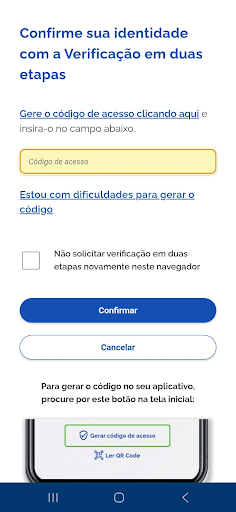
\includegraphics[height=4cm]{imagens/codigo_acesso.png}
    \caption{Geração de código divergente}
    \label{fig:prob1}
\end{subfigure}
\hfill
\begin{subfigure}{0.3\textwidth}
    \centering
    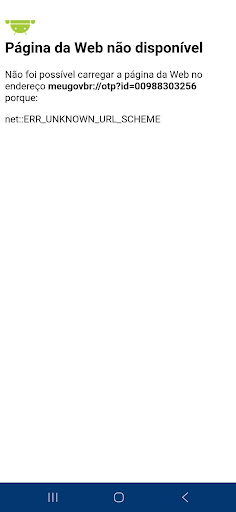
\includegraphics[height=4cm]{imagens/erro_link.png}
    \caption{Erro no redirecionamento}
    \label{fig:prob2}
\end{subfigure}
\hfill
\begin{subfigure}{0.3\textwidth}
    \centering
    
\includegraphics[height=4cm]{imagens/carregamento.png}
    \caption{Carregamento das consultas}
    \label{fig:prob3}
\end{subfigure}

\vspace{0.3 cm}

\begin{subfigure}{0.3\textwidth}
    \centering
    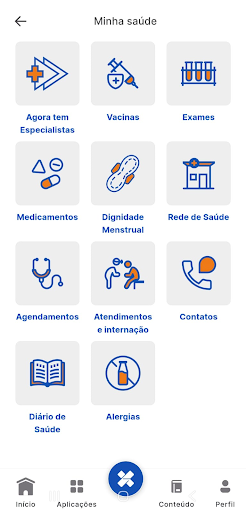
\includegraphics[height=4cm]{imagens/historico.png}
    \caption{Nomenclatura do histórico}
    \label{fig:prob4}
\end{subfigure}
\hfill
\begin{subfigure}{0.3\textwidth}
    \centering
    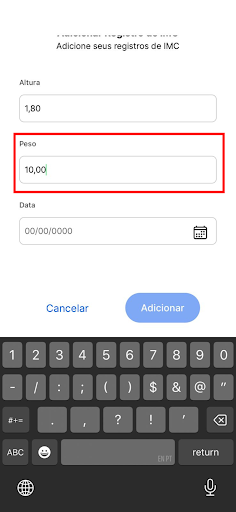
\includegraphics[height=4cm]{imagens/peso_imc.png}
    \caption{Campo de peso limitado}
    \label{fig:prob5}
\end{subfigure}
\hfill
\begin{subfigure}{0.3\textwidth}
    \centering
    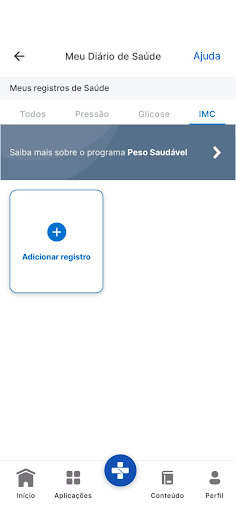
\includegraphics[height=4cm]{imagens/imc_nao_registrado.png}
    \caption{IMC não registrado}
    \label{fig:prob6}
\end{subfigure}

\caption{Telas correspondentes aos problemas catastróficos identificados}
\label{fig:problemas_catastroficos}
\end{figure*}

 \subsection{Resultados do teste de usabilidade} \label{sec:resultados_usabilidade}

Os testes de usabilidade empíricos permitiram avaliar a interação dos usuários com a interface do aplicativo Meu SUS Digital, com o objetivo de identificar o grau de acessibilidade e usabilidade da plataforma em relação ao público em processo de envelhecimento, buscando mostrar em que medida princípios de Interação Humano-Computador (IHC) foram efetivamente aplicados em seu design.

 A Tabela~\ref{tab:perfil_usuarios}, retrata o perfil demográfico e o comportamento digital dos cinco participantes envolvidos no teste, a fim de mapear suas experiências anteriores e correlacionar com os resultados adquiridos da validação da interface.  
 
\begin{table}[htbp]
\centering
\caption{Perfil demográfico e contexto tecnológico dos participantes}
\label{tab:perfil_usuarios}
\small
\begin{tabularx}{\textwidth}{|c|c|c|X|}
\hline
\textbf{Código} & \textbf{Idade} & \textbf{Gênero} & \textbf{Perfil e Contexto Tecnológico de Uso} \\ \hline
\textbf{P01} & 52 anos & Feminino & Uso diário de redes sociais (WhatsApp/Facebook), envio de áudios e dependência de ícones consolidados. \\ \hline
\textbf{P02} & 61 anos & Feminino & Uso diário de redes sociais e uso corporativo para transações bancárias. \\ \hline
\textbf{P03} & 70 anos & Feminino & Uso diário de redes sociais, envio de áudios e forte uso de ícones conhecidos. \\ \hline
\textbf{P04} & 59 anos & Masculino & Uso rotineiro de WhatsApp e aplicativos bancários para transações. \\ \hline
\textbf{P05} & 63 anos & Feminino & Uso regular de WhatsApp/Facebook com auxílio constante do filho.  \\ \hline
\end{tabularx}
\end{table}

A avaliação consistiu na observação de aspectos quantitativos e qualitativos, com o monitoramento do tempo de execução, além do registro de barreiras encontradas durante a realização das três atividades previstas no cenário de teste. Posto isto, os resultados com o tempo de execução e os aspectos comportamentais dos usuários serão apresentados a seguir organizados por tarefas, a fim de facilitar a compreensão dos dados. 

\begin{table*}[htbp]
\centering
\footnotesize
\caption{Tempo de execução por tarefa no Teste de Usabilidade}
\label{tab:teste_usabilidade}
\begin{tabular}{|c|c|c|c|}
\hline
\textbf{Participante} & \textbf{Tarefa 1 (Comprovante)} & \textbf{Tarefa 2 (Histórico)} & \textbf{Tarefa 3 (IMC)} \\
\hline
P01 & 2min10s & 3min20s & 5min20s \\
\hline
P02 & 1min08s & 4min09s & 3min09s \\
\hline
P03 & 3min10s & 1min10s & 4min00s\textsuperscript{*} \\
\hline
P04 & 2min15s & 1min09s & 4min15s \\
\hline
P05 & 4min13s & 4min00s & 6min00s \\
\hline
\end{tabular}

\vspace{0.2cm}
\footnotesize{\textsuperscript{*}Tarefa não concluída pela participante (insucesso).}
\end{table*}

\subsubsection{Exportar comprovante de vacina}
A primeira tarefa apresentou melhor taxa de sucesso na conclusão, porém a tarefa revelou problemas de eficiência no uso da aplicação. Diante da realização da tarefa,a participante \textit{}{P01} concluiu a ação sem dificuldades, essa facilidade ocorreu, principalmente, por conta da localização estratégica dos ícones principais e pelo design intuitivo da plataforma. Entretanto, a participante \textit{P02} enfrentou uma barreira técnica severa logo no início devido à lentidão da aplicação, impactando diretamente na fluidez da experiência do usuário.

Além do mais, os outros voluntários apresentaram problemas acerca da visibilidade dos elementos de interface: o participante \textit{P03} cometeu 3 erros de clique em locais incorretos devido à falta de destaque do botão de baixar o certificado; já o \textit{P04} manifestou dificuldades para localizar tanto a opção de todas as vacinas quanto o comando de exportação; e o \textit{P05} enfrentou dificuldades semelhantes, tendo dificuldade tanto para localizar o menu de vacinas quanto para identificar o botão de exportação entre os demais ícones não clicáveis presentes na página.

\subsubsection{Verificar o histórico de atendimentos}
A busca pelo histórico de atendimentos identificou várias inconsistências na interface do aplicativo, o que é evidenciado pelo tempo de execução, mostrado na tabela~\ref{tab:teste_usabilidade}, e pelas dificuldades relatadas pelos usuários. 

A participante \textit{P03} apresentou maior agilidade na execução, registrando apenas 1 erro e 1 pedido de ajuda. Entretanto, o restante da amostra enfrentou dificuldades relacionadas à visibilidade e à nomenclatura dos elementos no sistema, \textit{P01} sofreu com a falta de visibilidade gerada pelo ocultamento da funcionalidade sob o botão "Ver tudo", incorrendo em 2 erros e necessitando de 2 solicitações de suporte, já \textit{P04} relatou demora no carregamento da página, além da dificuldade na identificação do ícone que representa a função, além disso \textit{P05} teve sua busca dificultada pela presença de uma janela de "autoidentificação", que obstruiu a localização do menu contendo os ícones de serviços principais do aplicativo.

Todavia, a interação de \textit{P02} foi a mais comprometida entre os participantes, a tarefa foi prejudicada por interrupções contínuas de \textit{pop-ups} de permissão do sistema, que interromperam o fluxo cognitivo da participante, além de ambiguidade textual entre os rótulos "Histórico de Consulta" e "Agendamento", levando a repetidas confusões e a um perceptível desgaste ao longo da tentativa.

\subsubsection{Calcular o IMC na aba "Meu Diário de Saúde"}
A terceira tarefa foi, claramente, a mais complexa para o público-alvo, conforme evidenciado pelos tempos de execução apresentados na Tabela ~\ref{tab:teste_usabilidade}. Vale destacar a performance da participante \textit{P03}, que não conseguiu concluir a atividade devido ao cansaço mental após cometer cinco erros e realizar três pedidos de ajuda sem sucesso.

Embora os demais voluntários tenham conseguido finalizar a tarefa, eles também enfrentaram diversos obstáculos durante o percurso, o \textit{P01} apresentou a mesma dificuldade da tarefa anterior que consistia na falta de clareza do mapa do aplicativo, que mantinha o recurso escondido em "Ver tudo", e acabou sendo redirecionado acidentalmente para um site externo de uma campanha de saúde, além de relatar a ausência de rótulos claros para as unidades de medida solicitadas, registrando 5 erros ao longo da tentativa, além disso \textit{P02} confundiu o ícone do diário de saúde com o botão de acessibilidade do sistema e enfrentou interrupções recorrentes por telas de permissão durante a navegação.


Ademais, problemas críticos relacionados aos campos de entrada de dados também foram amplamente registrados; \textit{P04} e \textit{P05} relataram forte ambiguidade no campo obrigatório de ``data'', por não especificar o formato ou o tipo de data esperado (nascimento, consulta ou registro). Além disso, a participante \textit{P05} ainda foi redirecionada erroneamente para uma página meramente informativa ao tocar em ``saiba mais sobre IMC'', evidenciando a pouca ênfase visual dada ao botão real de inserção dos dados . Por fim, \textit{P01}, \textit{P02} e \textit{P04} confirmaram a ausência completa de \textit{feedback} ou mensagens de confirmação após o preenchimento dos dados de peso e altura, gerando incerteza quanto ao sucesso do registro mesmo entre os que completaram a tarefa, o que corrobora diretamente os problemas já identificados durante a realização da avaliação heurística .

Em suma, os resultados dos testes de usabilidade revelam que o aplicativo apresenta sérias barreiras de acessibilidade para o público maduro. Vale destacar que, enquanto tarefas localizadas na tela inicial foram concluídas com maior facilidade, fluxos mais complexos, envolvendo menus ocultos e preenchimento de dados, geraram alta taxa de erros e até desistências, demonstrando que a usabilidade da aplicação não é efetiva na prática \cite{barbosa2010ihc}. Portanto, essas dificuldades empíricas confirmam os problemas de navegação e a falta de \textit{feedback} que já haviam sido apontados na avaliação heurística, reforçando a necessidade latente de um \textit{redesign} na interface da plataforma.

 \subsection{Aplicação do Método de Inspeção Semiótica (MIS)}

Com a finalidade de complementar os achados da avaliação heurística e do teste
de usabilidade, aplicou-se o Método de Inspeção Semiótica (MIS) sobre o
aplicativo Meu SUS Digital, com foco na funcionalidade ``Meu Diário de
Saúde''. Diferentemente dos métodos anteriores, centrados na identificação de
problemas pontuais de interação, o MIS permitiu investigar como a
metacomunicação entre a equipe de design e o usuário final se manifesta por
meio dos signos presentes na interface, evidenciando pressupostos do
projetista que podem não corresponder ao repertório do público idoso.

\subsubsection{Passo 1: Preparar a Inspeção Semiótica}

Como fontes de informação foram utilizadas a própria interface do aplicativo
Meu SUS Digital (versão mobile), a documentação de ajuda disponível dentro do
aplicativo e os achados já produzidos nas avaliações anteriores (avaliação
heurística e teste de usabilidade). O escopo definido para a inspeção
compreendeu a jornada de navegação iniciada pelo login na conta gov.br,
seguida pela verificação do histórico de consultas, pela realização do
cálculo do Índice de Massa Corporal (IMC) na funcionalidade ``Meu Diário de
Saúde'' e pela consulta às vacinas tomadas.

A meta-mensagem inicial de comunicação, do ponto de vista do projetista para
o usuário final, pode ser assim formulada:

\emph{[Aqui está o meu entendimento sobre quem é você]: você é um cidadão
brasileiro que se preocupa com a sua saúde e deseja manter-se em dia com suas
vacinas e demais cuidados de saúde. Você já possui uma conta gov.br e busca
acompanhar informações de saúde de forma autônoma, estando familiarizado com
convenções básicas de aplicativos móveis, como toques em botões e listas
roláveis, e sendo capaz de reconhecer ícones e atalhos por associação visual,
sem necessidade de treinamento prévio.}

\subsubsection{Passo 2: Analisar os Signos Metalinguísticos}

Os signos metalinguísticos identificados ao longo da jornada concentram-se,
sobretudo, nas telas de autenticação e na tela inicial do aplicativo. Na tela
de login gov.br, destaca-se a instrução textual associada ao campo de CPF
(``Digite seu CPF para criar ou acessar sua conta gov.br''), que orienta
explicitamente o usuário quanto à finalidade do campo, além do selo ``Sua
conta será prata'', que qualifica antecipadamente a consequência de se optar
pelo ``Login com seu banco''. Já na tela inicial do Meu SUS Digital, a
mensagem ``Você não está logado. Entre com o Gov.br e acesse todas as
aplicações do novo Meu SUS Digital.'' constitui uma metamensagem explícita,
que informa o estado atual do sistema (usuário não autenticado) e instrui
diretamente a ação necessária para prosseguir (Figura~\ref{fig:signos-metalinguisticos}).

\begin{figure}[h]
  \centering
  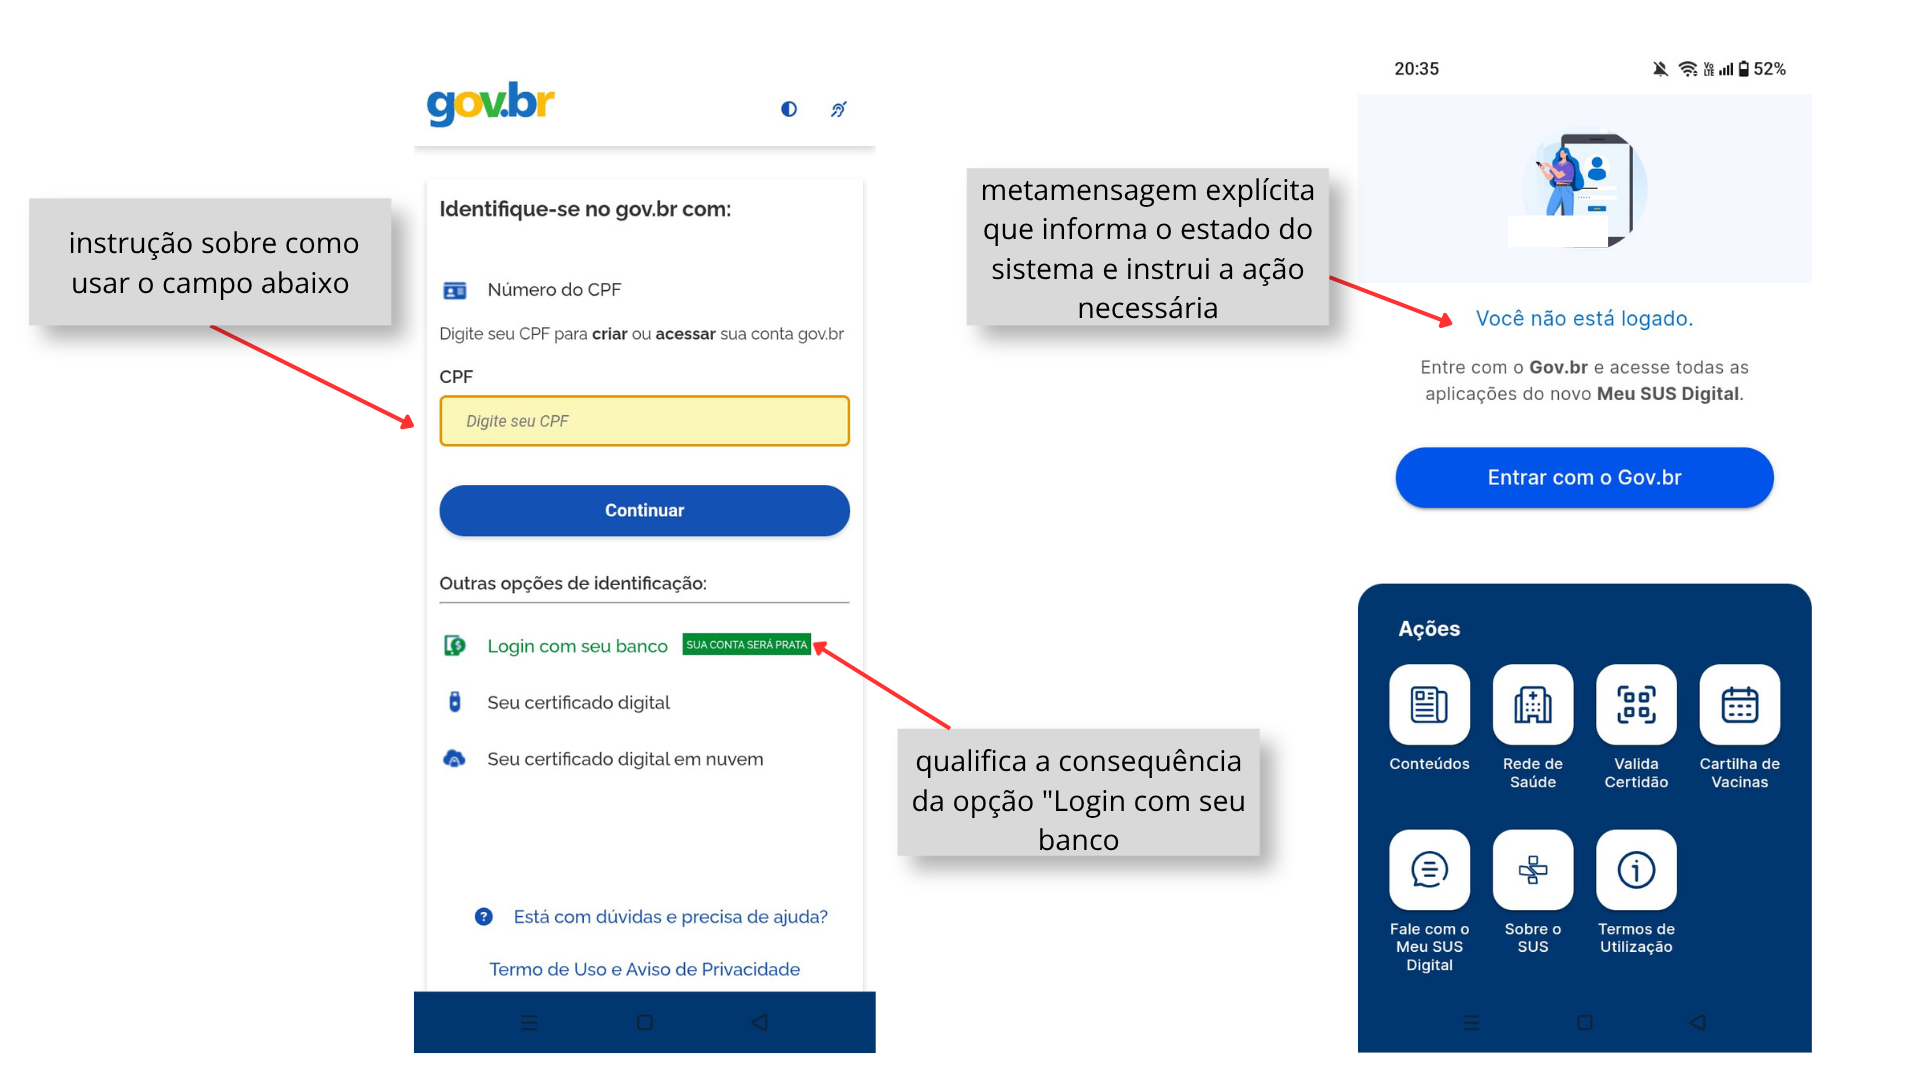
\includegraphics[width=0.8\linewidth]{imagens/signos_metalinguisticos.png}
  \caption{Signos metalinguísticos identificados nas telas de login gov.br e
  Início do aplicativo Meu SUS Digital.}
  \label{fig:signos-metalinguisticos}
\end{figure}

\emph{[O que eu aprendi que você quer ou precisa fazer, de que forma e por
quê]: você precisa se autenticar corretamente para acessar suas informações
de saúde, e pode ter dúvidas pontuais sobre qual campo preencher ou qual
método de login escolher.}

\emph{[Este é o sistema que eu projetei para você e essa é a maneira pela
qual você pode ou deve utilizá-lo]: cada campo e cada opção de autenticação é
acompanhado de uma instrução textual direta, e o sistema informa
proativamente quando você ainda não está autenticado, indicando a ação
necessária.}

Esse padrão de comunicação explícita, no entanto, não se repete na tela
``Meu Diário de Saúde'': não foram localizados, ao longo da jornada de
registro de IMC, tooltips, textos explicativos ou ícones de informação
contextual associados às abas de categoria (Todos, Pressão, Glicose, IMC) ou
ao botão ``Adicionar registro'', restando apenas o link genérico ``Ajuda'',
posicionado no canto superior direito da tela.

\emph{[O que eu aprendi que você quer ou precisa fazer, de que forma e por
quê]: você precisa registrar e revisar indicadores de saúde por categoria, e
pode ter dúvidas específicas em pontos críticos como o preenchimento de um
novo dado.}

\emph{[Este é o sistema que eu projetei para você e essa é a maneira pela
qual você pode ou deve utilizá-lo]: caso surjam dúvidas, o link ``Ajuda''
está disponível a qualquer momento na parte superior da tela. Para as demais
interações, presume-se que o significado dos ícones e rótulos seja
suficiente, dispensando explicações adicionais.}

Essa discrepância entre etapas evidencia uma inconsistência na estratégia de
metacomunicação do aplicativo: enquanto o fluxo de autenticação comunica seu
estado e orienta a ação do usuário de forma explícita e redundante, a etapa
de registro de dados de saúde  identificada pela avaliação heurística como
catastrófica carece do mesmo nível de suporte metalinguístico, exigindo
que o usuário reconheça, por conta própria, que precisa de ajuda e interrompa
sua tarefa para buscá-la.

\subsubsection{Passo 3: Analisar os Signos Estáticos}

Na tela ``Minha saúde'', foram identificados como signos estáticos os blocos
de ícone e rótulo dispostos em grade (Medicamentos, Dignidade Menstrual, Rede
de Saúde, Agendamentos, Atendimentos e internação, Contatos, Diário de
Saúde, Alergias), nos quais o ícone e o rótulo comunicam a categoria por
associação visual direta, seguindo um padrão de apresentação repetido em
todos os blocos. Cabe destacar que, funcionalmente, esses blocos operam como
botões: ao serem tocados, conduzem o usuário a uma nova tela, o que também
permitiria interpretá-los como signos dinâmicos. Optou-se, contudo, por
classificá-los aqui como signos estáticos porque é o ícone, e não o efeito
de transição desencadeado pelo toque, o elemento analisado neste passo: o
ícone representa uma categoria de conteúdo de forma persistente,
independente da interação estar ou não em curso, sendo esse o critério que
define sua condição de signo estático. Esse mesmo princípio se mantém na
tela ``Vacinas'': o rótulo posicionado sobre cada cartão.

\begin{figure}[h]
  \centering
  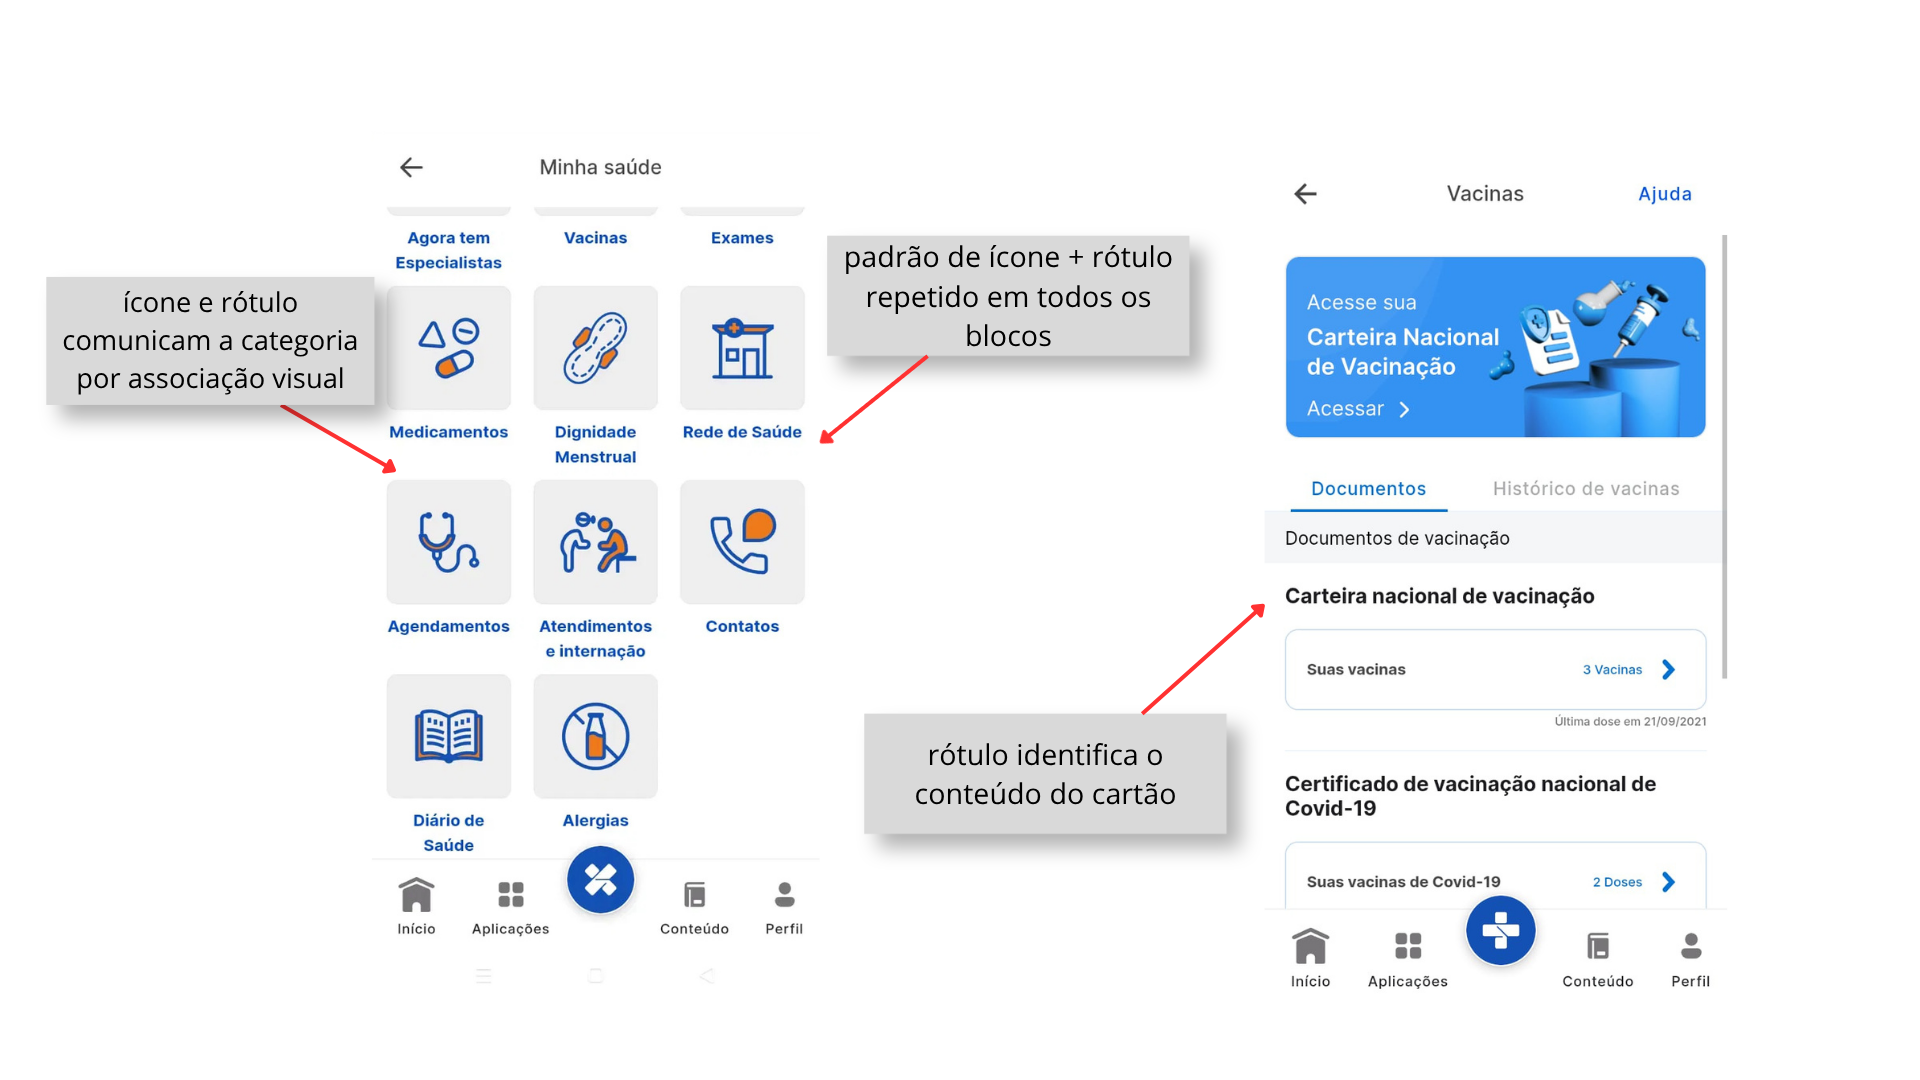
\includegraphics[width=0.8\linewidth]{imagens/signos_estaticos_diario_saude.png}
  \caption{Signos estáticos identificados nas telas Minha saúde e Vacinas do
  aplicativo Meu SUS Digital.}
  \label{fig:signos-estaticos}
\end{figure}

Já na tela ``Meu Diário de Saúde'', destacam-se como signos estáticos o
conjunto de abas de categoria (Todos, Pressão, Glicose, IMC) e o cartão azul
com a chamada ``Saiba mais sobre o programa Peso Saudável''.

\emph{[O que eu aprendi que você quer ou precisa fazer, de que forma e por
quê]: você precisa localizar rapidamente a categoria de informação de saúde
que deseja consultar, sem precisar navegar por menus profundos.}

\emph{[Este é o sistema que eu projetei para você e essa é a maneira pela
qual você pode ou deve utilizá-lo]: os ícones e rótulos de cada bloco
comunicam, por associação visual direta, a que tipo de conteúdo eles levam.
A aba ``IMC'' destacada em azul sinaliza qual categoria está selecionada no
momento, seguindo um padrão comum de navegação por abas.}



\subsubsection{Passo 4: Analisar os Signos Dinâmicos}

Os signos dinâmicos concentram os elementos que mais caracterizam a jornada
analisada, pois é por meio deles que o usuário avança de fato entre os
estados da interface. Foram identificados três signos dinâmicos principais,
apresentados na Figura~\ref{fig:signos-dinamicos}: (i) os atalhos por
categoria na tela ``Início'' (Agora tem Especialistas, Vacinas, Exames,
Medicamentos), que ao serem tocados transicionam para a tela de detalhe
correspondente; (ii) o link ``Ver tudo'', que expande a listagem de atalhos
disponíveis; e (iii) o botão ``Adicionar registro'' na tela ``Meu Diário de
Saúde'', posicionado como a ação central da tela, que ao ser tocado deveria
transicionar o estado da interface para o formulário de registro de um novo
dado de IMC.

\emph{[O que eu aprendi que você quer ou precisa fazer, de que forma e por
quê]: você precisa navegar entre categorias de informação e registrar novos
dados de saúde, e espera receber confirmação visual clara de que cada ação
foi executada com sucesso.}

\emph{[Este é o sistema que eu projetei para você e essa é a maneira pela
qual você pode ou deve utilizá-lo]: toque nos atalhos de categoria para
acessar o conteúdo correspondente; toque em ``Ver tudo'' para expandir a
lista completa; toque no botão circular ``+'' de ``Adicionar registro'' para
iniciar o preenchimento de um novo dado de saúde.}

\begin{figure}[h]
  \centering
  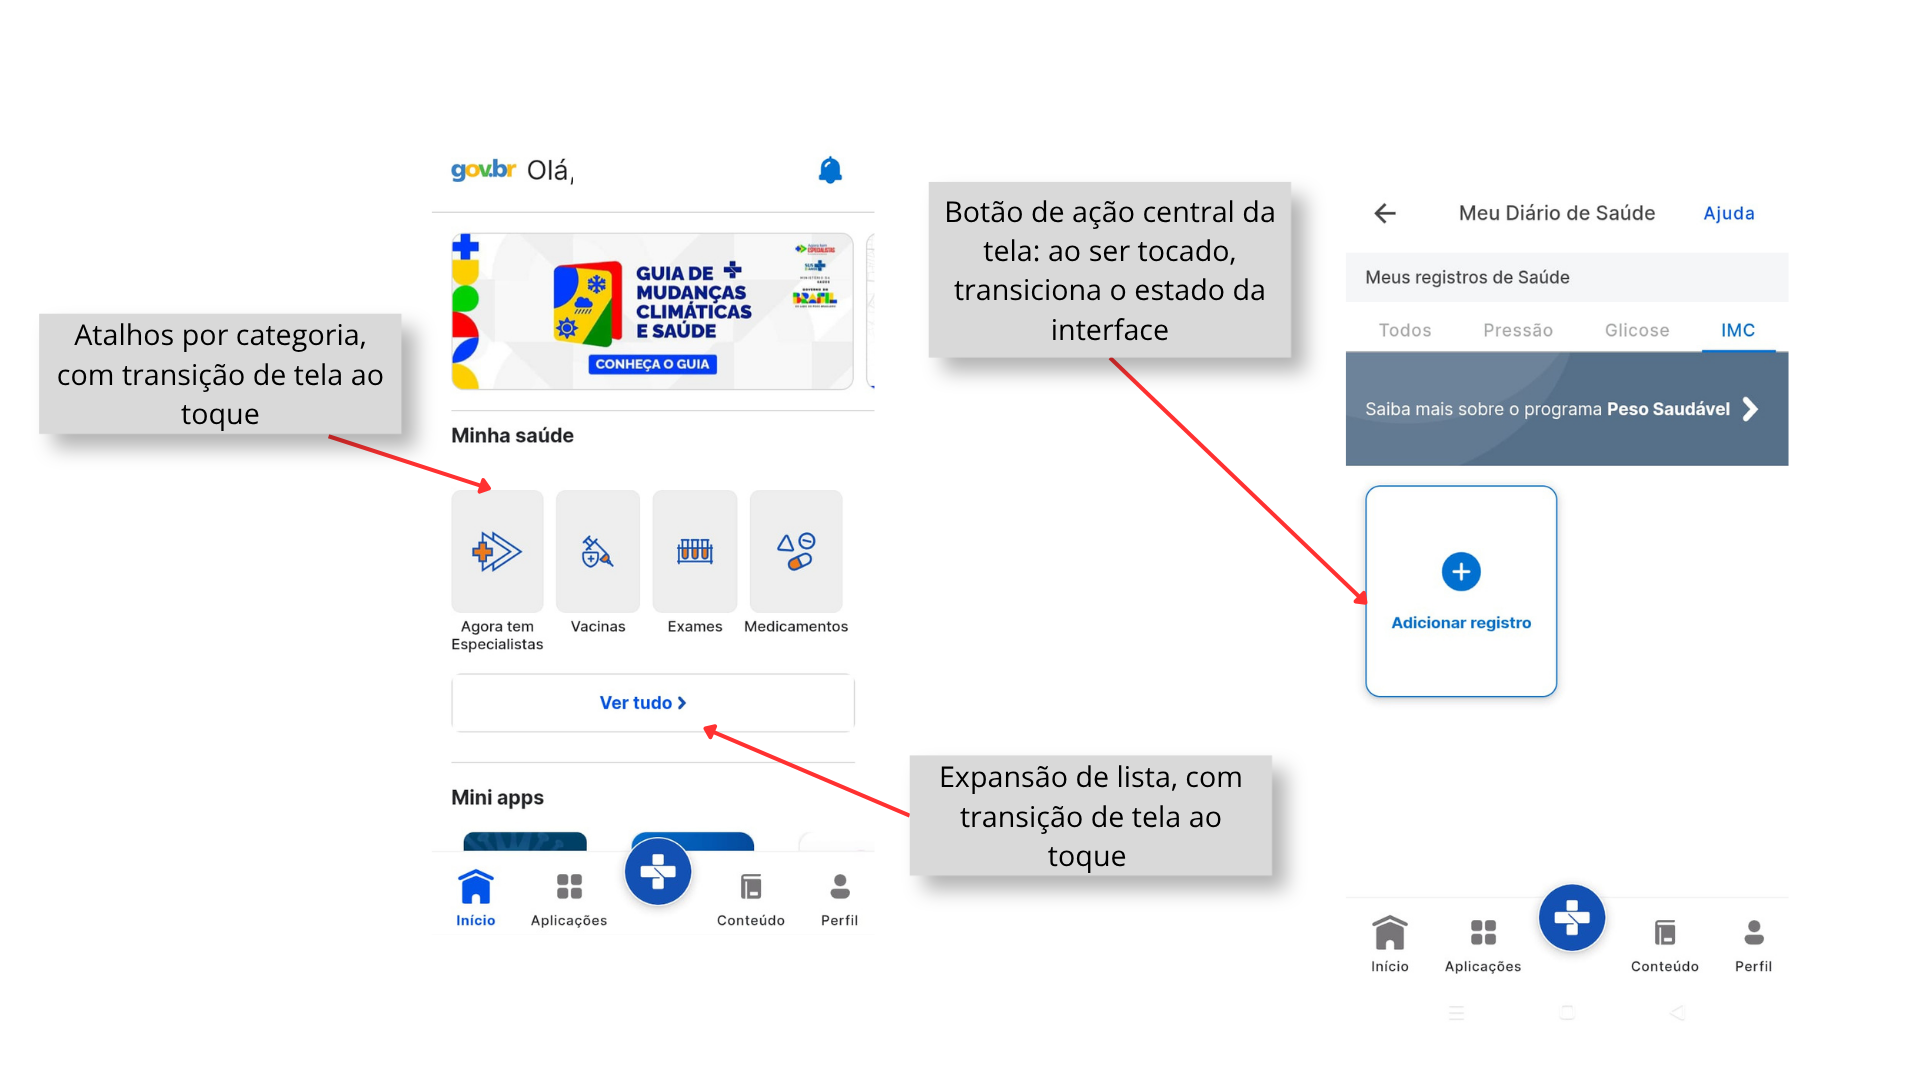
\includegraphics[width=0.8\linewidth]{imagens/signos_dinamicos_diario_saude.png}
  \caption{Signos dinâmicos identificados nas telas Início e Meu Diário de
  Saúde do aplicativo Meu SUS Digital.}
  \label{fig:signos-dinamicos}
\end{figure}

O botão ``Adicionar registro'' é o signo dinâmico de maior relevância para
este trabalho, pois é o ponto de entrada da tarefa em que a avaliação
heurística identificou o problema catastrófico de ausência de registro do
IMC. Embora o botão comunique com clareza, por meio de contraste de cor,
formato e posicionamento central, que se trata da ação principal da tela, a
inspeção não localizou, nas telas subsequentes ao seu acionamento, um signo
dinâmico equivalente que confirme ao usuário a conclusão bem-sucedida do
registro.

\subsubsection{Passo 5: Comparar}

Ao comparar as mensagens de metacomunicação levantadas nos passos anteriores,
observa-se coerência entre os signos estáticos e dinâmicos da tela
``Início'': os atalhos por categoria e o link ``Ver tudo'' comunicam de forma
redundante e consistente para onde cada toque irá levar o usuário, o que
favorece a intuitividade dessa etapa da jornada.

Entretanto, identifica-se uma quebra relevante de comunicabilidade no fluxo
que se inicia no botão ``Adicionar registro''. O sinal dinâmico de
início da ação (botão destacado, ícone ``+'', rótulo em negrito) , não há
correspondência de sinal ao final do fluxo: não há signo
dinâmico ou metalinguístico que confirme, na visão do usuário, que o registro
foi de fato salvo. Essa assimetria entre o início e o fim do fluxo de
metacomunicação explica, sob a ótica semiótica, por que o problema de
usabilidade identificado pela avaliação heurística (IMC não registrado mesmo
após preenchimento completo dos dados) tende a passar despercebido pela
própria equipe de design: o sistema comunica com força a intenção de
registrar, mas não comunica sua falha ou sucesso.

\subsubsection{Passo 6: Avaliar}

A aplicação do MIS permitiu identificar que a jornada analisada apresenta boa
comunicabilidade em suas etapas de autenticação e navegação inicial, com
redundância adequada entre signos estáticos, dinâmicos e metalinguísticos,
mas apresenta uma lacuna crítica de metacomunicação exatamente no ponto
identificado como catastrófico pela avaliação heurística: o registro de um
novo dado no ``Meu Diário de Saúde''. Essa convergência de achados, obtidos
por métodos distintos (inspeção especialista, teste com usuários reais e
inspeção semiótica), reforça a validade do problema identificado e evidencia
que sua causa-raiz não está apenas na execução técnica da funcionalidade, mas
na ausência de um signo de confirmação na interface.
 
 \subsection{Problemas selecionados para o \textit{redesign}}
 As telas  escolhidas para o \textit{redesign} são oriundas dos problemas catastróficos encontrados durante a avaliação heurística e comprovados durante a avaliação de usabilidade, visando mitigar os empecilhos encontrados na navegação da interface.   

 \subsubsection{Reestruturação das páginas de exportar comprovante de vacina}
Em relação à interface do aplicativo, buscou-se solucionar os problemas encontrados nas observações e inspeções realizadas. Para isso, retirou-se o \textit{banner} no topo da tela relacionado ao acesso à carteira nacional de vacinação e adicionou-se um botão que torna mais rápida a exportação das vacinas registradas, visando uma navegação mais eficiente. Além disso, foi criado um menu que permite ao usuário escolher de quais vacinas deseja gerar o comprovante para, em seguida, exportá-lo.

\begin{figure}[h]
  \centering
  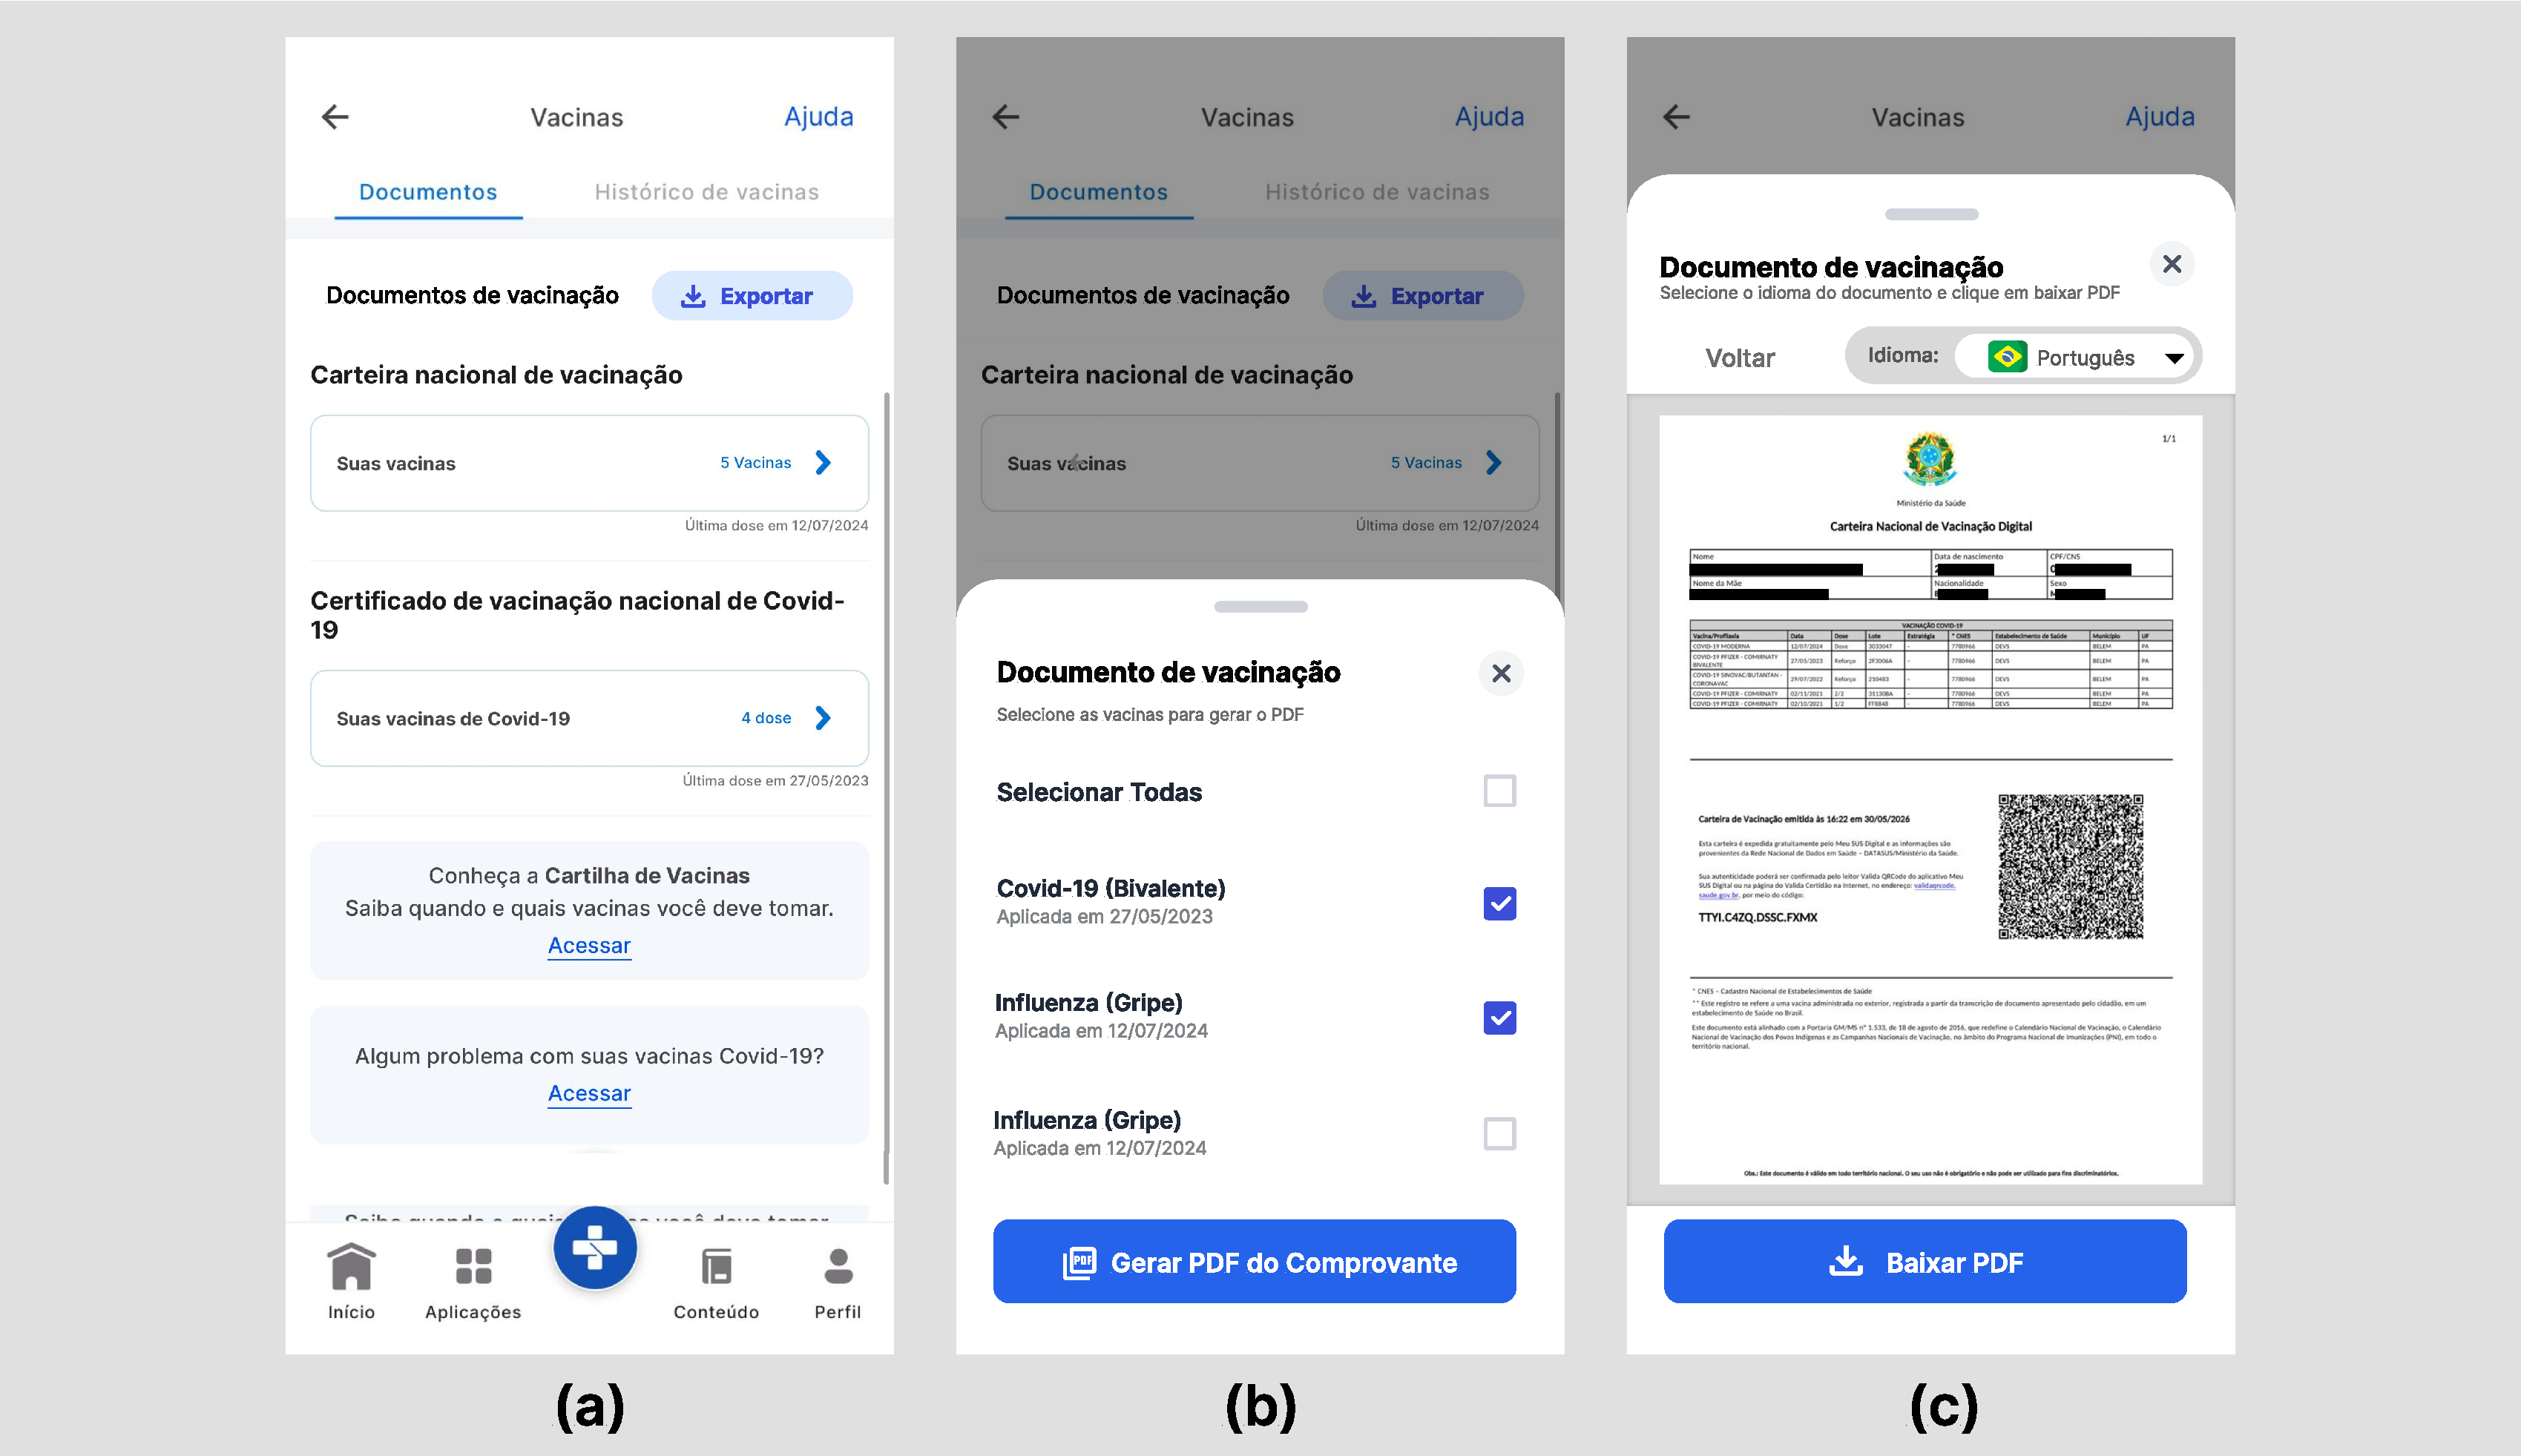
\includegraphics[width=0.8\linewidth]{imagens/redesign/Fluxo para exportar comprovante de vacinação.pdf}
  \caption{Redesign da tela de exportar comprovante de vacinação}
  \label{fig:signos-dinamicos}
\end{figure}

 \subsubsection{Reestruturação das páginas de IMC}

 A etapa de registrar o IMC apresentou-se como um dos principais desafios para os participantes dos testes de usabilidade na seção \ref{sec:resultados_usabilidade}. Nesse sentido, a reformulação dessa funcionalidade ganha um aspecto de maior urgência, a fim de tornar o acesso à interface mais acessível ao público-alvo do estudo. Portanto, mitigar aspectos como aumento excessivo de atenção para ícones não essenciais e reformular campos de preenchimento não descritivos tornaram-se prioridades no processo do \textit{redesign}.

\begin{figure}[h]
  \centering
  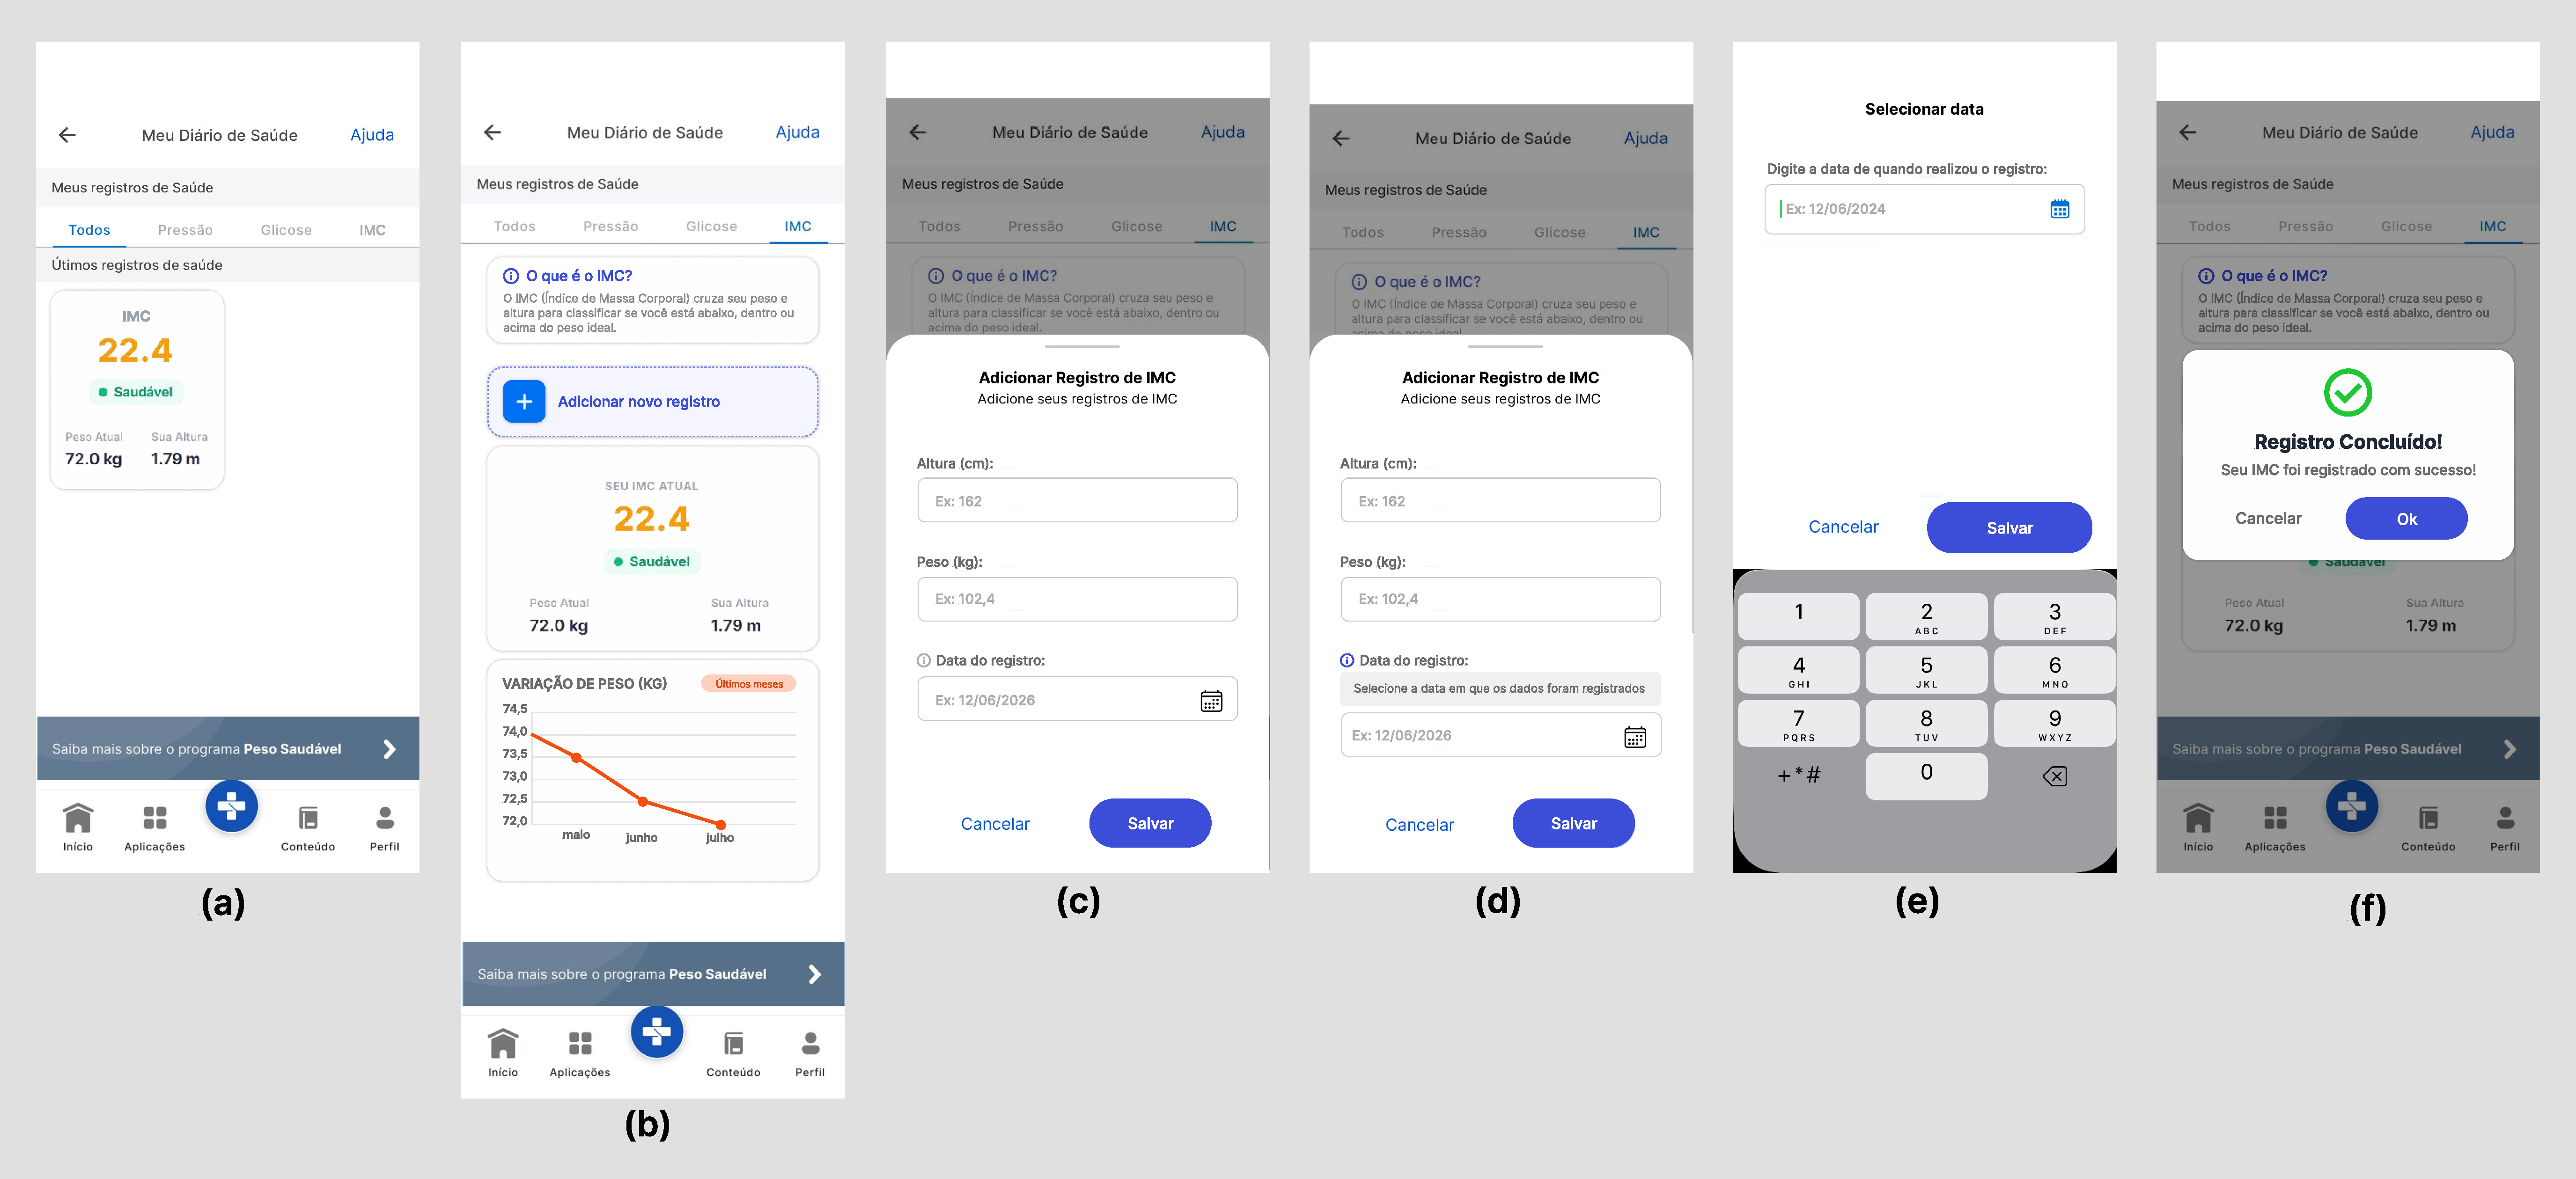
\includegraphics[width=0.8\linewidth]{imagens/redesign/Fluxo para cadastrar IMC.pdf}
  \caption{Redesign da tela de exportar comprovante de vacinação}
  \label{fig:signos-dinamicos}
\end{figure}

% \begin{figure*}[htbp]
%     \centering
%     \begin{subfigure}{0.3\textwidth}
%         \centering
%         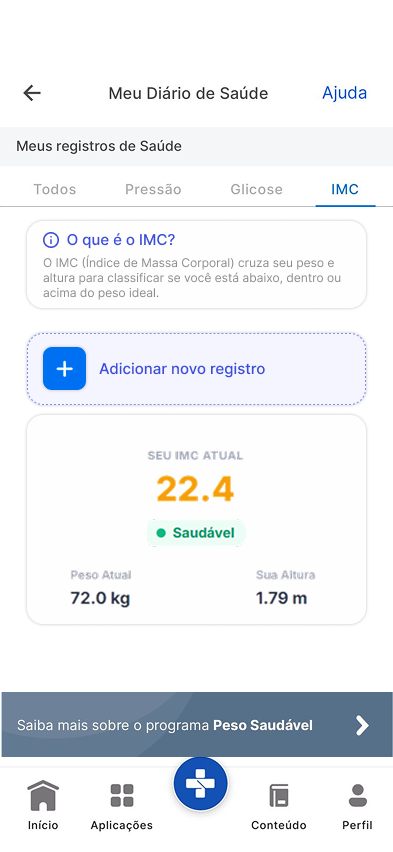
\includegraphics[height=4cm]{imagens/redesign/IMC - Adicionar Registro (Modificada).png}
%         \caption{Tela inicial de IMC modificada}
%         \label{fig:tela_imc_inicial_modificada}
%     \end{subfigure}
%     \hfill
%     \begin{subfigure}{0.3\textwidth}
%         \centering
%         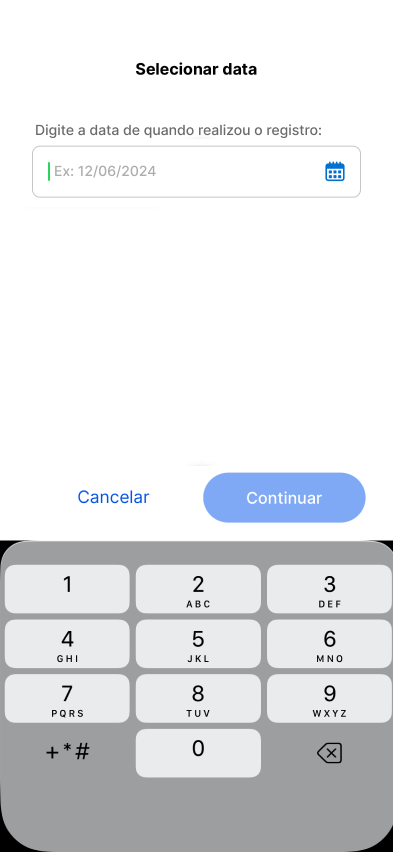
\includegraphics[height=4cm]{imagens/redesign/IMC - Data do Registro (Modificado).png}
%         \caption{Tela modificada de inserção de data de IMC}
%         \label{fig:tela_imc_data_modificada}
%     \end{subfigure}
%     \hfill
%     \begin{subfigure}{0.3\textwidth}
%         \centering
%         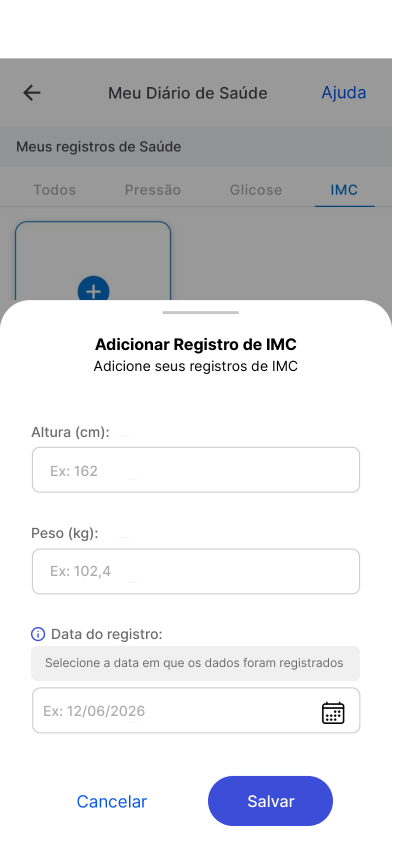
\includegraphics[height=4cm]{imagens/redesign/IMC - Inserção Registro 2 (Modificado).png}
%         \caption{Tela modificada de inserção de registro com dica de IMC}
%         \label{fig:tela_imc_insercao_modificada}
%     \end{subfigure}
    
%     \caption{Telas correspondentes aos redesignes do objeto de estudo}
%     \label{fig:telas_redesign}
% \end{figure*}

 A priori, a tela inicial da página de IMC demonstrou-se uma barreira cognitiva considerável para que os usuário direcionassem a sua atenção para adicionar o registro. A visualização do botão de adição de registro era menos destacada na tela em relação ao ícone de redirecionamento para a tela de informações sobre ICM, causando uma confusão comum. Em consequência, o usuário via-se confuso diante da sobrecarga visual e direcionava-se ao botão de redirecionamento e perdia-se diante da troca de tela inesperada. Assim, o primeiro redesign dessa tela é a alteração da posição do botão de informações para que o mesmo seja um elemento com menos destaque, além de uma redução na sua área da tela ocupada como visto na imagem 7b unida a um maior realce sobre as informações e o botão de adição de registro.

 Outrossim, um enclave rotineiro durante os testes de usabilidade foi o preenchimento dos campos obrigatórios para o cálculo do índice. Nesse sentido, os campos originais apresentavam poucas informações importantes como a unidade métrica do campo e a forma de preenche-lo, ocasionando em sérios desvios de usabilidade da aplicação. Desse modo, o redesign surge com o intuito de adicionar as unidades de medida para cada campo, demonstrar exemplos de preenchimento para que o usuário possa basear-se e adicionar a opção de entender melhor o que o campo significa para uma inserção de dados mais precisa demonstrada na imagem 7d.

 Por fim, a etapa de preenchimento do campo de data do registro apresentou conflito na utilização do calendário de seleção original. Esse conflito no entendimento ocorre devido a divergência do campo em relação aos outros, criando uma camada maior de complexidade e de surpresa ao usuário, frustrando o seu uso de forma ideal além do texto ser pouco explicativo na explicação do campo. Para esse fim, optou-se por retirar completamente a funcionalidade de calendário embutido e utilizar apenas a inserção numérica da data no lugar em conjunto com a utilização do separador "/" automaticamente conforme a digitação do usuário, assim como um texto mais explicativo sobre o que o campo refere-se, sendo o resultado dessa mudança mostrado na imagem 7e.

 \subsubsection{Reestruturação das página de menu}
Nesta etapa, foram realizadas pequenas mudanças incrementais, mas cruciais para a melhoria da experiência do usuário. A primeira alteração consistiu na substituição do termo 'atendimentos e internações' por 'histórico clínico', atendendo a uma dificuldade recorrente relatada pelos participantes dos testes. Além disso, adicionou-se uma barra de pesquisa na parte superior da tela, visando agilizar o acesso às funcionalidades do sistema.

\begin{figure}[h]
  \centering
  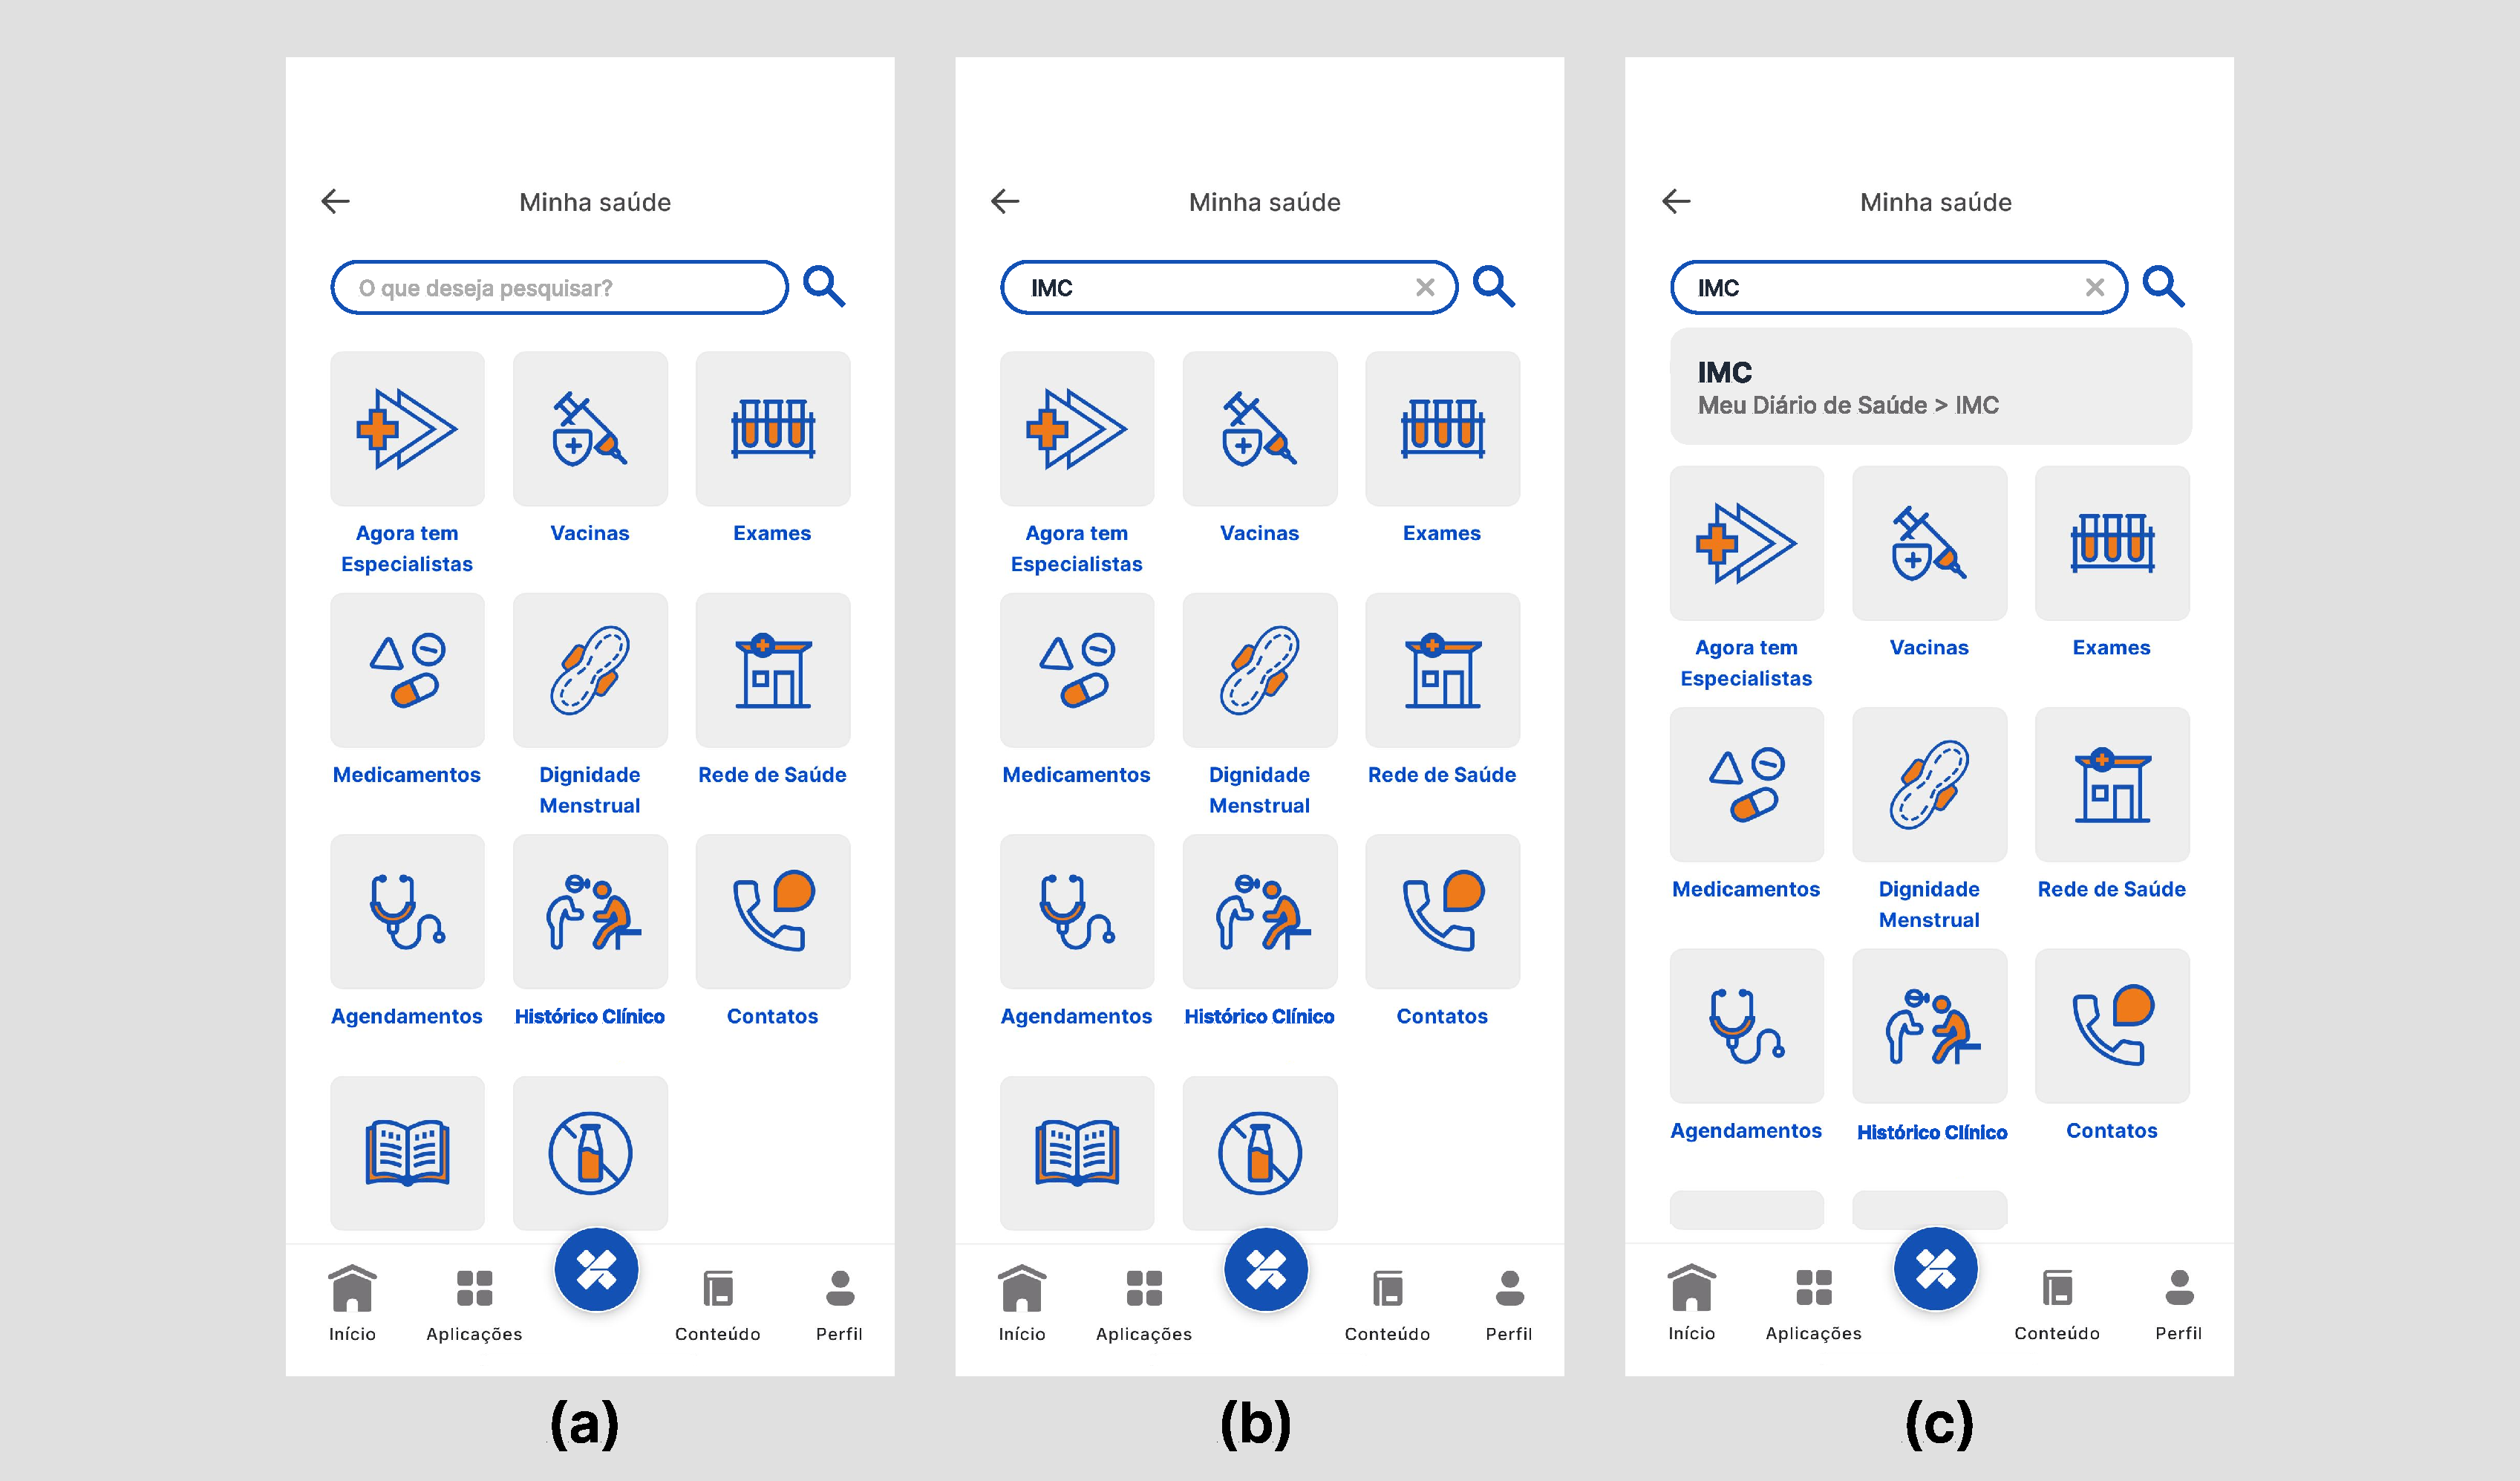
\includegraphics[width=0.8\linewidth]{imagens/redesign/Fluxo para pesquisar no menu.pdf}
  \caption{Redesign da tela de exportar comprovante de vacinação}
  \label{fig:signos-dinamicos}
\end{figure}
 
\subsection{Resultados do teste de usabilidade com protótipo}
Tendo em vista a necessidade de verificar se as mudanças acrescentadas na interface melhoraram a usabilidade, foi realizado um teste com dois usuários, seguindo os passos indicados em seções anteriores. Na tabela \ref{tab:perfil_usuarios_redesign}, é possível verificar o perfil demográfico e a sua afinidade com a tecnologia.

\begin{table}[htbp]
\centering
\caption{Perfil demográfico e contexto tecnológico dos participantes}
\label{tab:perfil_usuarios_redesign}
\small
\begin{tabularx}{\textwidth}{|c|c|c|X|}
\hline
\textbf{Código} & \textbf{Idade} & \textbf{Gênero} & \textbf{Perfil e Contexto Tecnológico de Uso} \\ \hline
\textbf{P01} & 62 anos & Feminino & Uso diário de redes sociais (WhatsApp/Facebook/Instagram) e baixa familiaridade com aplicativos do Governo, mas utiliza aplicativos bancários para transações. \\ \hline
\textbf{P02} & 87 anos & Feminino & Uso diário de redes sociais (WhatsApp/Facebook/Instagram), baixa familiaridade com aplicativos do Governo. \\ \hline
\end{tabularx}
\end{table}

Em relação a Tabela \ref{tab:teste_usabilidade_redesign}, é possível verificar o tempo que cada participante teve para completar cada tarefa. Vale destacar que diferente do primeiro teste de usabilidade realizado, estes fluxos se encontram isolados, sem conexão direta com a totalidade do aplicativo, podendo se um fator que impactou no tempo cronometrado. Apesar disso, é possível inferir que houve uma melhora significativa no tempo para completar as tarefas.

Para comprovar isso, calcularam-se as médias de tempo do primeiro e do segundo testes em relação às tarefas de calcular o IMC e exportar o comprovante de vacinação. Em seguida, foram mensuradas a melhoria percentual. Como resultado, a primeira tarefa apresentou uma evolução de 69,71\% no tempo de conclusão e na segunda 55,28\%.

\begin{table*}[htbp]
\centering
\footnotesize
\caption{Tempo de execução por tarefa no Teste de Usabilidade}
\label{tab:teste_usabilidade_redesign}
\begin{tabular}{|c|c|c|c|}
\hline
\textbf{Participante} & \textbf{Tarefa 1 (Comprovante)} & \textbf{Tarefa 2 (Pesquisa)} & \textbf{Tarefa 3 (IMC)} \\
\hline
P01 & 31s & 20s & 1min09s \\
\hline
P02 & 1min03s & 1min45s & 2min55s \\
\hline
\end{tabular}
\end{table*}

Por fim, as participantes sugeriram pequenas melhorias no protótipo. Em relação ao fluxo de exportar o comprovante de vacinação, foi sugerido que as letras do documento em pré-visualização fossem maiores, facilitando a leitura antes do download. Além disso, houve a sugestão de melhorar o contraste dos textos no menu superior do fluxo de cálculo do IMC. Apesar desses pontos, as usuárias gostaram das mudanças, com destaque para o \textit{card} informativo sobre o IMC.
 
\section{Considerações finais}
Este trabalho teve como objetivo avaliar a usabilidade e a acessibilidade do aplicativo governamental "Meu SUS Digital" com foco na perspectiva de uso do público em processo de envelhecimento, a partir da aplicação combinada de três métodos: Avaliação Heurística, Teste de Usabilidade e Método de Inspeção Semiótica (MIS). A partir do uso dessas ferramentas, foi identificado que o sistema possui problemas significativos de usabilidade, muitos dos quais impactam diretamente a autonomia do idoso, contribuindo para o aumento da segregação tecnológica desses indivíduos \cite{wiei}.

A partir desses achados, foi realizado um processo de \textit{redesign} da interface, o qual foi submetido a um novo teste de usabilidade. Apesar da pequena amostragem utilizada nesse segundo teste, foi notória a mitigação de parte dos problemas identificados anteriormente, evidenciando que as melhorias foram parcialmente eficazes.


\bibliographystyle{sbc}
\bibliography{sbc-template}

\end{document}